%% Standard-Vorspann
\documentclass[a4paper,11pt,twoside]{report}
\usepackage{ngerman}  
\usepackage[utf8]{inputenc}                
%\usepackage[latin1]{inputenc}
\usepackage[T1]{fontenc}
\usepackage[fleqn]{amsmath}
\usepackage{mathtools}
\usepackage{bm}
\DeclarePairedDelimiter\ceil{\lceil}{\rceil}
\DeclarePairedDelimiter\floor{\lfloor}{\rfloor}

%% Auf Schriftart Palatino umschalten
\usepackage{mathpazo}
\usepackage[scaled=.95]{helvet}
\usepackage{courier}
\usepackage[figuresright]{rotating}
%% fast immer benoetigte Pakete
\usepackage{acronym}
\usepackage{amssymb, amsthm}
\usepackage{alltt}
\usepackage{latexsym}
\usepackage{makeidx}
\usepackage{textcomp}
\usepackage{rotating}
\usepackage{color}
\usepackage[table]{xcolor}
\usepackage{caption}
\usepackage{listings}
\usepackage{verbatim}
\usepackage{fancyhdr}
\usepackage{graphicx}
\usepackage{subcaption}
\usepackage{thmtools}
\declaretheorem[style=Definition, title=Definition, numberwithin=chapter]{dfn}
\newtheorem{axiom}{Axiom}
\usepackage{tikz}
\usepackage{multirow}
\usepackage[natbib,maxnames=3,style=numeric,backend=bibtex,sortlocale=de]{biblatex}
\addbibresource{bibtex/literature.bib}
\DeclareBibliographyCategory{fullcited}
\usepackage{listings}
\usepackage[hang]{footmisc}
\usepackage{chngcntr}
\counterwithout{footnote}{chapter}
\setlength{\footnotemargin}{0pt}
\usepackage{url}
\renewcommand\UrlFont{\sffamily\slshape}
\usepackage{nicefrac}
\usepackage{units}
\usepackage{minibox}
\pdfminorversion=7
\usepackage{emptypage}
\usepackage{hyperref}

%% spezielles Zeug
\usepackage{Abschlussarbeit}


%
\chapter{Abk\"urzungsverzeichnis}

% ======================================================================
% Declare acronyms
% ======================================================================

\begin{acronym}
	\acro{ARRI}[ARRI]{Arnold \& Richter Cine Technik GmbH \& Co. Betriebs KG}
	\acro{fpga}[FPGA]{Field Programmable Gate Array}
	\acro{fra}[FRA]{FPGA Resource Abstraction}
	\acro{geo}[Geo Framework]{Geometrie Framework}
	\acro{gui}[GUI]{grafische Benutzeroberfläche}
	\acro{ioctl}[IOCTL]{IO Control}
	\acro{mfd}[MFD]{Multifunction Device}
	\acro{rec}[REC]{Aufnahme}
	\acro{pid}[PID]{Prozesskennung}
	\acro{smpte}[SMPTE]{Society of Motion Picture and Television Engineers}
	\acro{sdi}[SDI]{Serial Digital Interface} gemäß \ac{smpte} 292M \cite{smpte}
	\acro{xbar}[Xbar]{Crossbar}
\end{acronym}



%% Index erzeugen
\makeindex

%% jetzt geht's los
\begin{document}
\raggedbottom
\hypersetup{
	colorlinks,
	citecolor=black,
	filecolor=black,
	linkcolor=black,
	urlcolor=black
}

\definecolor{mygreen}{rgb}{0,0.6,0}
\definecolor{mygray}{rgb}{0.5,0.5,0.5}
\definecolor{mymauve}{rgb}{0.58,0,0.82}

\lstset{language=C,
		basicstyle=\footnotesize,
		commentstyle=\color{mygreen},
		keywordstyle=\color{blue},
		numbers=left,
		numbersep=5pt,
		numberstyle=\tiny\color{mygray},
		breakatwhitespace=false,
		tabsize=2,	
		frame=single, %todo ja oder nein??
		breaklines=true}
\captionsetup[lstlisting]{font=it,
						  position=below,
					  	  belowskip=0.5cm}

%% Die Datei "Vorspann.tex"  bitte ausf�llen!
% Vorspann der Arbeit
%


\includegraphics[width=45mm]{pictures/Hochschule_Muenchen_Logo.png}
\hfill

\includegraphics[width=45mm]{pictures/ARRI_AG_Corporate_Logo.png}

\vspace*{20mm}
\begin{center}
{\large Hochschule f\"ur angewandte Wissenschaften M\"unchen}\\
{\large Fakult\"at f\"ur Elektrotechnik und Informationstechnik}\\
{\large Bachelorstudiengang Elektrotechnik und Informationstechnik}\\

\vspace*{15mm}
{\huge Bachelorarbeit }    %% oder Masterarbeit
\\

\vspace*{10mm}
{\huge \bfseries{%
                      \par Modulare Ansteuerung eines FPGAs \"uber Software \par
}} 


\vspace*{15mm}
{\Large abgegeben von %
                      Maren Konrad 
%%                    Vorname Name
} 
\\
\end{center}

\vfill
{\large
\begin{tabbing}
\\
Bearbeitungsbeginn: \hspace{3.5cm} \= %
					  12.08.2019
\\
Abgabetermin: \> \= %     
                      12.02.2020
%%                    durch Ende-Datum ersetzen
\\
lfd. Nr. gem\"a{\ss}  Belegschein: \> %
					  1883 
\\
\end{tabbing} }
\thispagestyle{empty}
\cleardoublepage


% Seite 2
\vspace*{20mm}
\begin{center}
{\large Hochschule f\"ur angewandte Wissenschaften M\"unchen}\\
{\large Fakult\"at f\"ur Elektrotechnik und Informationstechnik}\\
{\large Bachelorstudiengang Elektrotechnik und Informationstechnik}\\

\vspace*{15mm}
{\huge Bachelorarbeit }    %% oder Masterarbeit
\\

\vspace*{10mm}
{\huge \bfseries{%
		\par Modulare Ansteuerung eines bildverarbeitenden FPGAs "uber generische Kernelmodule \par
}} % deuscher Langtitel

\vspace*{10mm}
{\huge \bfseries{%
		\par Modular control of an image processing FPGA via generic kernelmoduls \par
}} % englischer Langtitel

\vspace*{15mm}
{\Large abgegeben von %
	Maren Konrad 
	%%                    Vorname Name
} 
\\
\end{center}

\vfill
{\large
	\begin{tabbing}
		\\
		Bearbeitungsbeginn: \hspace{3.5cm} \= %     
		12.08.2019
		%%                    durch Start-Datum ersetzen
		\\
		Abgabetermin: \> %     
		12.02.2020
		%%                    durch Ende-Datum ersetzen
		\\
		lfd. Nr. gem\"a{\ss}  Belegschein: \> %
		1883
		%%                    durch Lfd. Nr. ersetzen
		\\
		Betreuer (Hochschule M\"unchen): \> %         
		Prof. Dr. Gerhard Schillhuber
		%%                    hier den Prof. eintragen
		\\
		Betreuer (Extern): \> %         
		Anton Hattendorf
\end{tabbing} }
\thispagestyle{empty}
\cleardoublepage

% Seite 3
\thispagestyle{empty}
Erkl\"arungen des Bearbeiters:\\
\\
Name: Konrad \\
Vorname: Maren \\

1) Ich erkl\"are hiermit, dass ich die vorliegende Bachelorarbeit selbst\"andig verfasst
und noch nicht anderweitig zu Pr\"ufungszwecken vorgelegt habe.

S\"amtliche benutzte Quellen und Hilfsmittel sind angegeben, w\"ortliche und sinngem\"a{\ss}e Zitate sind als solche gekennzeichnet.
\vspace{15mm}

\begin{tabbing}
	M\"unchen, den \today \hspace{10mm} \= \rule{60mm}{0.5pt}\\
	\> {\small Unterschrift}
\end{tabbing}
\vspace{15mm}

\vfill
2) Der Ver\"offentlichung der Bachelorarbeit stimme ich hiermit \textbf{NICHT} zu.
\vspace{15mm}

\begin{tabbing}
	M\"unchen, den \today \hspace{10mm} \= \rule{60mm}{0.5pt}\\
	\> {\small Unterschrift}
\end{tabbing}

\vfill
\cleardoublepage

%Seite 4

\begin{center}
{\Large \bfseries{ Kurzfassung }}\\
\end{center}

%% Hier die Kurzfassung in Deutsch einf�gen
%In dem vorliegenden Bericht geht es um die Verbesserung einer Kamerasoftware. Es wird hierzu eine Abstraktionsebene vorgestellt, die aus mehreren Modulen besteht. Um das Verst\"andnis zu erleichtern wird au\ss{}erdem eine kurze Einf\"uhrung zur Bildkette gegeben und anschlie\ss{}end auf ausgew\"ahlte Module eingegangen. Durch die Abstraktionsebene wird die \"Ubersichtlichkeit und Erweiterung der Software in Zukunft erleichtert werden.

%todo noch ein bissl mehr dazu schreiben
In dem vorliegenden Bericht geht es um die Verbesserung einer Kamerasoftware im Zusammenspiel mit der Hardware. Es wird hierzu eine Abstraktionsebene vorgestellt, welche die Zugriffe von der Software auf den FPGA \"ubersichtlicher und einfacher gestalten soll. Der Zugriff auf die Hardware findet aktuell direkt \"uber die Adresse statt und soll abstrahiert werden, sodass die Software lediglich den Namen ben\"otigt um auf des richtige Modul zuzugreifen. Zum Erleichtern des Verst\"andnis wird ein kurzer \"Uberblick \"uber die aktuelle Implementierung und eine kurze Einf\"uhrung zur Bildkette gegeben. Au\ss{}erdem wird auf das Betriebssystem Linux und ben\"otigte Komponenten eingegangen. Im Anschluss wird die Implementierung der Abstraktionsebene n\"aher erkl\"art. Die Wartbarkeit und die Erweiterung der Software soll durch die Abstraktionsebene in Zukunft erleichtert werden.


Dieser Bericht ist f\"ur Leser aus dem Bereich der Elektrotechnik geschrieben.

\vspace*{5mm}
\begin{center}
{\Large \bfseries{ Abstract }}\\
\end{center}

%% Hier die Kurzfassung in Englisch ein
%This report handle the improvement of an camera software. For this, an abstraction level will be introduce, which consists out of a few modules. At first there is a short intorduction to the image processing chain to make the understanding easier and then go into details of selected modules. Because of the abstraction level the clarity and extensions of the software will be easier in future. 

This report decribes the improvement of an camera software in interaction with the hardware. For this, an abstraction level will be introduced, which should simplify and clearer the accesses from the software to the FPGA. Currently the access to the hardware is directly via  an address. This should be abstract, so that the software only needs the name of an module to access it. It is given a overview at the current implementation and a short introduction to the image chain. Besides the basics of the operation system Linux and the required components are described. Afterwards the implementation of the abstraction level is explained more detailed. In the future the maintainability and extension of the software will be easier because of the abstraction layer.


This report targets readers having an electric engineering background.

\pagenumbering{Roman} 	
\renewcommand{\thechapter}{\Roman{chapter}} 

\cleardoublepage
%% Inhaltsverzeichnis
\tableofcontents
\clearpage



  

\chapter{Abk\"urzungsverzeichnis}

% ======================================================================
% Declare acronyms
% ======================================================================

\begin{acronym}
	\acro{ARRI}[ARRI]{Arnold \& Richter Cine Technik GmbH \& Co. Betriebs KG}
	\acro{fpga}[FPGA]{Field Programmable Gate Array}
	\acro{fra}[FRA]{FPGA Resource Abstraction}
	\acro{geo}[Geo Framework]{Geometrie Framework}
	\acro{gui}[GUI]{grafische Benutzeroberfläche}
	\acro{ioctl}[IOCTL]{IO Control}
	\acro{mfd}[MFD]{Multifunction Device}
	\acro{rec}[REC]{Aufnahme}
	\acro{pid}[PID]{Prozesskennung}
	\acro{smpte}[SMPTE]{Society of Motion Picture and Television Engineers}
	\acro{sdi}[SDI]{Serial Digital Interface} gemäß \ac{smpte} 292M \cite{smpte}
	\acro{xbar}[Xbar]{Crossbar}
\end{acronym}



%% Hier kommt der eigentlich Text der Arbeit
%% sinnvoll ist, f�r jedes Kapitel eine eigene 
%% Datei zu nehmen, verk�rzt die Zeit beim LaTeX-Durchlauf
%% Erst am Schluss alle Dateien verwenden.

\chapter{Einleitung}

\section{\acl{ARRI}}
Die Bachelorarbeit fand bei der Firma \acl{ARRI} statt. Gegründet wurde die Firma 1917 und auch noch über 100 Jahren Firmengeschichte liegt der Hauptsitz von \ac{ARRI} noch immer in München. 
Weltweit sind mittlerweile um die 1500 Mitarbeiter angestellt und die Firma ist einer der führenden Hersteller und Lieferanten in der Film- und Fernsehindustrie.

Die \ac{ARRI} Gruppe teilt sich in die folgenden fünf Geschäftsbereiche ein: Kamerasysteme, Licht, Postproduktion, Verleihservice und Operationskamerasysteme für die Medizin. \cite{arricorpinfo}

Das Thema dieser Bachelorarbeit wurde im Bereich Kamerasysteme in der Forschungs- und Entwicklungsabteilung erarbeitet.

\section{Kontext}
Um einen Überblick über das Umfeld der Arbeit zu bekommen, werden zunächst ein paar Grundlagen und auch die Funktionsweise einer Kamera betrachtet.


\subsection{Entwicklungsplattform}
Als Erstes soll auf die Zielplattform eingegangen werden. Die Wahl der Kamera ist auf eine \ac{ARRI} AMIRA gefallen, da die Entwicklungsumgebung durch vorherige Arbeit bekannt ist. Zusätzlich ist sie nicht die aktuellste Kamera der Firma und somit ohne Probleme verfügbar. 
Die AMIRA ist eine vielseitige Kamera, die für eine Einmannbedienung ausgelegt ist. Zusätzlich ist sie mit einem Audioboard ausgestattet und aus diesem Grund bei Dokumentationsfilmen und der elektronischen Berichtserstattung gerne verwendet. Zum Beispiel wird die \ac{ARRI} AMIRA bei Sportveranstaltungen der National Football League (NFL) in Amerika eingesetzt.\cite{arrinewsamira} 

\begin{figure}[!hbtp]
	\centering
	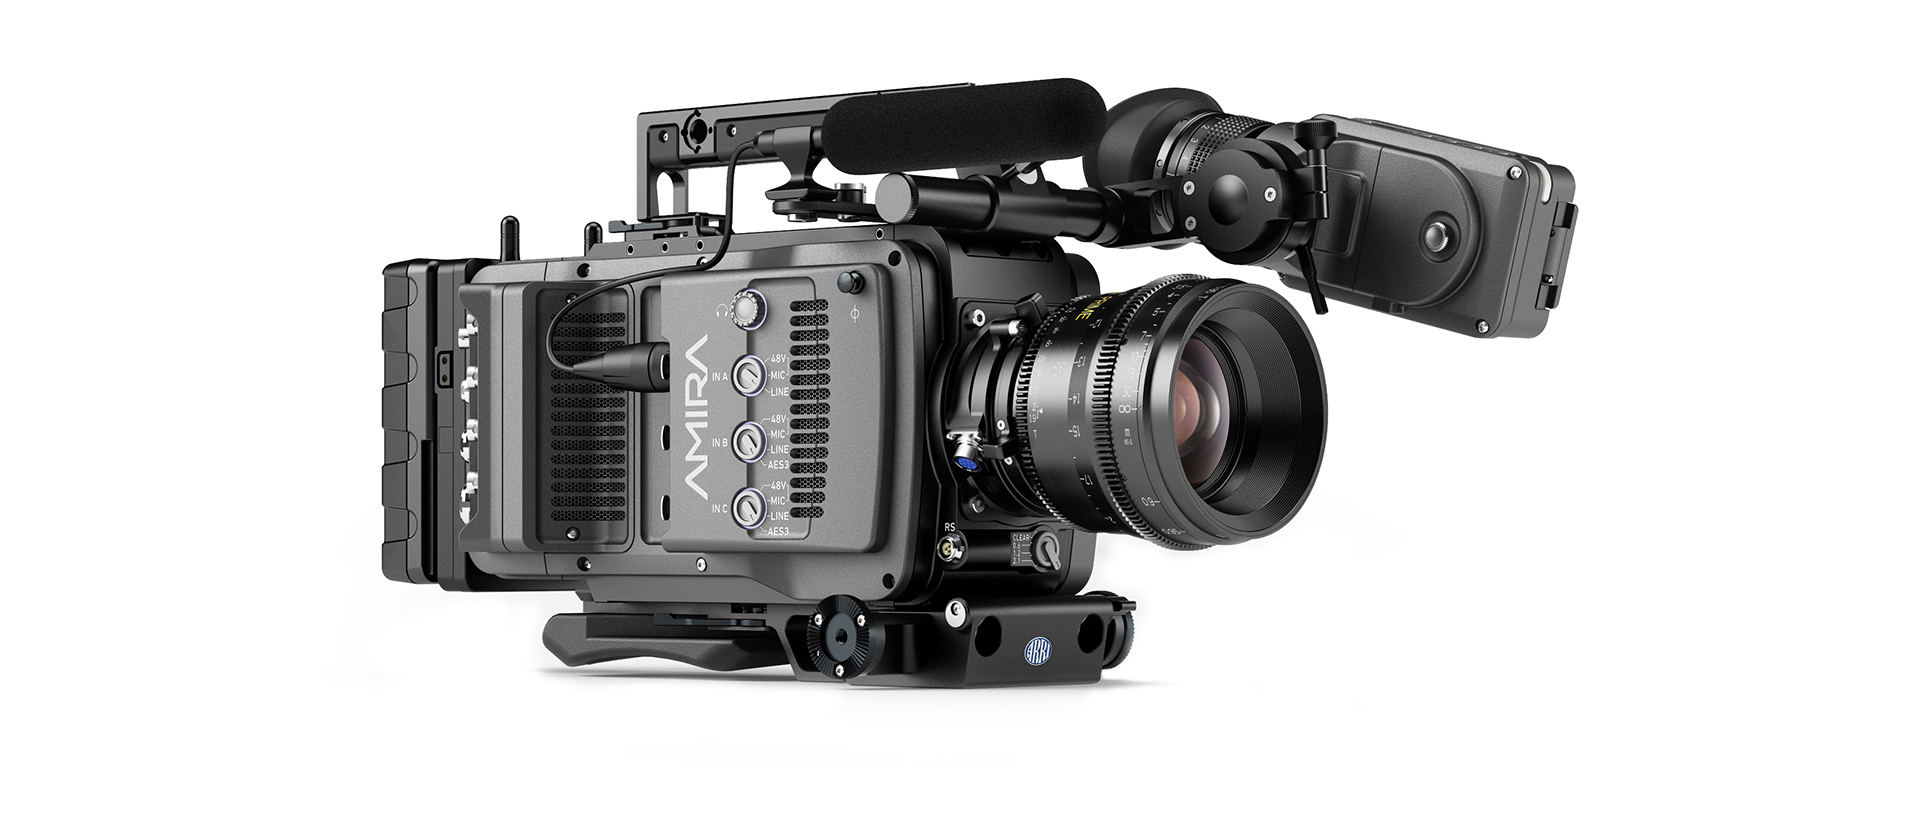
\includegraphics[width = 0.7\linewidth]{pictures/amira-product-image-data.jpg}
	\hspace*{0\textwidth}
	\caption{ARRI AMIRA}
	\caption*{siehe \cite{arriamira_bild}}
	\label{fig:amira}
\end{figure}  

Für Spielfilm- und Serienproduktionen wird auch manchmal die \ac{ARRI} AMIRA eingesetzt, wodurch das breite Einsatzspektrum der Kamera noch deutlicher wird.
Als Beispiele sind hier der bayrische Eberhofer Krimi \glqq Sauerkrautkoma\grqq{} \cite{arrikrimi}, die Netflixserie \glqq The Ivory Game\grqq{} \cite{imdbivory} oder auch das Fernsehmagazin \glqq The Grand Tour\grqq{} \cite{imdbtour} zu nennen.
 
Die Kamera ist ein wichtiger Bestandteil in der Entwicklungsarbeit, da das regelmäßige Testen von Änderungen unerlässlich ist, um die Funktionalität festzustellen und grobe Fehler rechtzeitig zu erkennen.

\subsection{Bildkette}
In jeder Kamera wird das Eingangsbild von einem Sensor aufgenommen. Durch die Verarbeitungskette werden die Bilder vom Eingang bis zum Ausgang geleitet. In dieser Arbeit wird eine schematische Bildkette (siehe Abbildung) zur Veranschaulichung weiter detailliert. Von der Quelle bis zu Senke läuft das Bild durch verschiedene Module, die für die Anpassung des Bilds sorgen. Die Ausgänge sind in diesem Fall die \ac{rec} und das \ac{sdi}.

\begin{figure}[!hbtp]
	\centering
	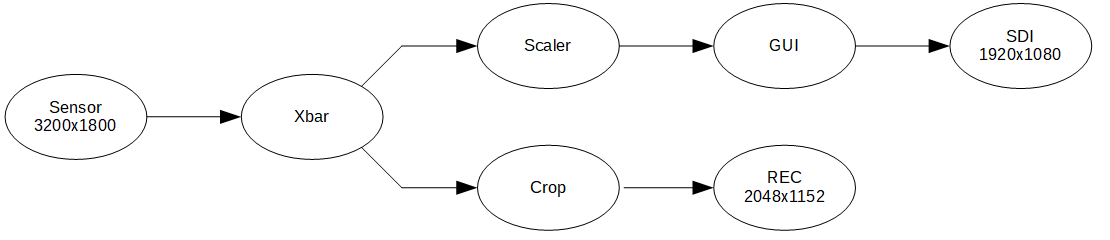
\includegraphics[width = \linewidth]{pictures/2019-11-17_Bildkette.png}
	\smallskip
	\caption{Schematische Bildkette}
	\label{fig:bild}
\end{figure} 

Direkt nach dem Sensor geht das Bild durch eine \ac{xbar}, hier wird das identische Bild in zwei Bildpfaden weitergeführt. Für die \acl{rec} wird das Bild im Crop zugeschnitten, damit wird nur ein bestimmter Bildausschnitt aufgezeichnet. In dem anderen Bildpfad wird, mithilfe des Scalers, das Bild kleiner skaliert. Nachdem eine grafische Benutzeroberfläche hinzugefügt worden ist, wird das Bild am \ac{sdi} ausgegeben. Hier ist, durch die Skalierung, das komplette Sensorbild einschließlich der eingefügten Oberfläche zu sehen.

In dieser Arbeit wird nur das \ac{fpga}-Modul \ac{xbar} softwareseitig implementiert, da weitere Module sonst den Umfang der Arbeit überschreitet.

\subsection{Implementierung}
Bevor auf das erarbeitete Konzept eingegangen wird, soll kurz auf die Funktionsweise der Kamera und die aktuelle Implementierung eingegangen werden.

Die bildverarbeitende Hauptfunktionalität liegt im \ac{fpga}. Hier werden die Module entsprechend der Bildkette angeordnet und verbunden. Durch die Software werden bei den \ac{fpga} Modulen entsprechende Einstellungen vorgenommen.

Damit die Einstellungen auch zu dem Sensorbild passen, werden alle Module des \ac{fpga}s in dem \ac{geo} abgebildet. Das objektorientierte Framework führt hauptsächlich Berechnungen der Bildgrößen und Offsets durch. Nach der Änderung einer Größe in der Quelle oder Senke werden alle Module in der abgebildeten Frameworkbildkette geupdatet und entsprechend der voreingestellten Parameter werden die Größen neu berechnet. In dem Update werden verschiedenen Funktionen aufgerufen, welche die Register im \ac{fpga} entsprechend der Einstellungen gesetzt.

\subsection{Problematiken}\label{sec:prob}
In der aktuellen Implementierung liegen verschiedene Probleme vor, die durch ein neues Framework eliminiert werden soll.

Zum Einen muss bei den Zugriff auf ein Modul immer der \ac{fpga} gesperrt werden. Dadurch kann es passieren, dass es einen oder zwei Frames dauert, bis alle Einstellungen in der Bildkette aktuell sind. Bei einem Livebild der Kamera ist dies besonders störend, da man die aktuelle Änderung erst später sieht. Da man beim Aufnehmen keine Änderungen am Sensorbild vornehmen kann fällt das Problem hier nicht ins Gewicht.

Des weiteren müssen die Adressen für die \ac{fpga} Module händisch eingetragen werden. Die Fehleranfälligkeit steigt dadurch natürlich weiter, da es passieren kann, dass die Software, Einstellungen an eine Adresse schreibt, hinter der kein Modul liegt. In schlechtesten Fall werden die Register eines anderen Modules beschrieben und es kommt zum Fehlerfall in der Bildkette.

Auch die Länge der Register wird in der aktuellen Implementierung nicht weiter berücksichtigt. So kann es dann passieren, dass über ein Register hinweg geschrieben wird. Auch dann kommt es zum Fehlerfall in der Bildkette, da andere Einstellungen überschrieben werden. 

Da die Fehlerfälle im normalen Umgang mit der Kamera auftreten können und somit in Produktionen zu Ausfällen sorgen, ist es wichtig die Probleme zu beheben.

%todo gloasar: framework, Dateideskriptoren, Handle, Middleware
\section{Konzept}
Die Probleme in der aktuellen Implementierung (siehe Kapitel~\ref{sec:prob}) sollen durch ein neues Framework behoben werden, zusätzlich sollen die Zugriffe der Software auf den \ac{fpga} übersichtlicher und wartbarer gestaltet werden.

\begin{figure}[!hbtp]
	\centering
	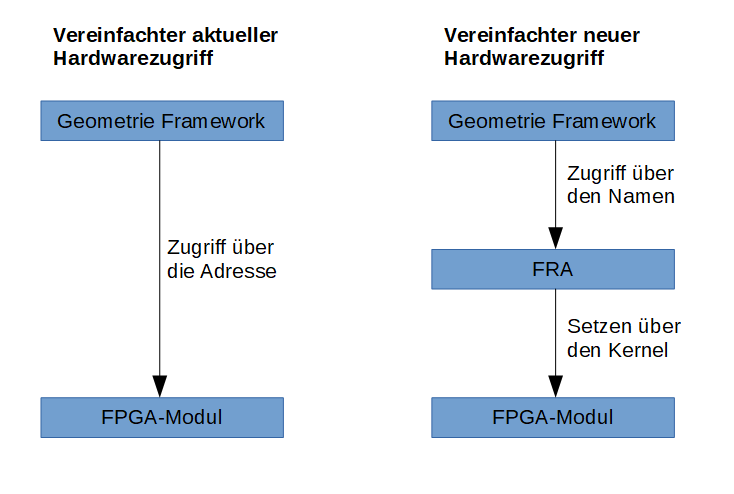
\includegraphics[width = 0.9\linewidth]{pictures/2019-11-17_ImplementierungNewvsOld.png}
	\smallskip
	\caption{Vereinfachte Darstellung des Zugriffs auf den \ac{fpga} in der aktuellen und der neuen Implementierung}
	\label{fig:newvsold}
\end{figure} 



Aktuell benötigen die Zugriffe auf den \ac{fpga} jedes Mal die Adressen der Module. Dadurch wird die Fehlersuche in diesen Teilen der Software extrem kompliziert und aufwendig. Durch eine weitere Abstraktionsebene soll eine modulare Ansteuerung möglich werden und so die direkten Hardwarezugriffe über die Adressen aus dem Hauptcode eliminiert werden. In dem \ac{fra} werden die Module im Kernel als Gerät angelegt und über Dateideskriptoren greift die Software auf den \ac{fpga} zu.


Die Geräte werden mit der Adresse, der Größe, dem Namen und Type des dahinterliegenden Modul beim Initialisieren des Bildpfads angelegt. Dieser Teil soll generisch generiert werden, aber aufgrund von verschiedenen Abhängigkeiten überschreitet es den Umfang der Arbeit.


Über den Namen im vorhandenen \ac{geo} werden die Dateideskriptoren in der Software geöffnet und in einem Handle gespeichert. Damit wird im Hauptteil des Codes ein Zugriff ohne Adresse gewährleistet. Jeder laufende Prozess muss seinen eigenen Dateideskriptor öffnen und verwaltet somit sein eigenes Handle. Pro Gerät kann lediglich eine begrenzte Anzahl von Deskriptoren geöffnet werden, geregelt wird dies durch den Kernel. 
Bei jedem Schreib- oder Lesezugriff auf ein Register wird überprüft, ob dieser innerhalb der angegebenen Modulgröße liegt. Damit ist es nicht mehr möglich über ein Register hinweg zuschreiben und somit falsche Module zu beschreiben.


Durch die neue Abstraktionsebene soll die Wartbarkeit sowie die Erweiterung der Kamerasoftware in Zukunft ohne tiefere Kenntnisse vom \ac{fpga} durch unterschiedliche Entwickler möglich werden.



%\section{Hinführung zum Thema}\label{sec:thema}
%Damit die Kamera einwandfrei funktioniert müssen Firmware und Software zusammenspielen. Im \ac{geo} werden die verschiedenen Module aus dem \ac{fpga} abgebildet und entsprechend der Kameraeinstellungen die Bildgrößen berechnet. 

%In der Software werden dann in verschiedenen Funktionen die einzelnen Register im \ac{fpga} entsprechend gesetzt. Durch die aktuelle Implementierung können keine Module gleichzeitig im \ac{fpga} geupdatet werden. 

%todo plural!
%Damit eine modulare Ansteuerung möglich wird, soll eine weitere Abstraktionsebene erstellt werden. Dieses sogenannte \ac{fra} soll die einzelnen Module im Kernel darstellen und entsprechend aus dem Userspace über \ac{ioctl} angesprochen werden können. Zusätzlich werden dann die direkten Hardwarezugriffe aus dem Hauptcode eliminiert. 

%Durch die neue Abstraktionsebene soll die Wartbarkeit sowie die Erweiterung der Kamerasoftware in Zukunft ohne tiefere Kenntnisse von \ac{fpga} durch unterschiedliche Entwickler möglich werden. 


%todo kernelversion der kamera und der zitate, erklärung das unterschiedliche nummern, da grundlegend identisch, neuere versionen allerdings mit mehr und ausfühlicheren kommentaren

\chapter{Grundlagen Linux} \label{sec:grund}
Zu Beginn sollen einige Grundlagen näher erläutert werden, die zum Erstellen der Arbeit essenziell waren.

\section{Linux - Kernel und Userspace}\label{sec:linux}
Da das Zielsystem auf Linux läuft, soll zunächst dieses Betriebssystem betrachtet werden. 
Im Herbst 1991 wurde die erste Version des Systems von Linus Torvalds veröffentlicht und der Gründer kümmert sich, mit Unterstützung, weiterhin um die Entwicklung des frei verfügbaren Betriebssystem. %todo quelle
 
Der Name Linux bezeichnet dabei eigentlich nur den Kern des Systems, auch Kernel genannt. Zusätzlich benötigt man noch System- und Anwendersoftware. Oft wird dieser Teil als Userspace zusammengefasst. \citep[S. 46]{plotner2012linux} 

Der Kernel hat verschiedene Aufgaben. Unter anderem ist er für die Prozess- und die Speicherverwaltung sowie das Gerätemanagement zuständig. \citep[S. 234]{schroder2009embedded} 

Im Normalfall hat der Nutzer aus dem Userspace keinen direkten Zugriff auf die Kernelfunktionen und der Hardware. Nur über Systemaufrufe, auch Syscalls, hat ein Programm im Userspace die Möglichkeit Änderungen an der Hardware zu kommunizieren beziehungsweise bestimmte Funktionen im Kernel zu nutzen. \citep[S. 124]{plotner2012linux} 
Die Brücke zwischen der Hardware und dem Benutzer stellt somit der Kernel da.


\section{\acl{ioctl}}\label{sec:ioctl_t}
Um ein zuverlässig arbeitendes Betriebssystem zu haben, muss der Speicherbereich von Kernel und der vom Userspace getrennt sein. \citep[S. 232]{schroder2009embedded}
Damit entsteht die Notwenigkeit zwischen Userspace und Kernel aktiv Daten auszutauschen. Die Anwendungen im Userspace können über das sogenannte Systemcall Interface auf die Funktionen im Kernel zugreifen. In einer Struktur vom Typ \textit{file\_operations} wird die Schnittstelle zu einem Treiber vorgegeben. In dieser Struktur werden treiberabhängige Funktionszeiger gespeichert. \citep[S. 249]{schroder2009embedded}

Im folgenden soll lediglich der Zeiger auf das \acf{ioctl} betrachtet werden, da dieser im weiteren Teil der Arbeit eine wichtige Rolle spielt.
Durch die \ac{ioctl} Methode wird dem Programmierer ein flexibles Werkzeug zur Verfügung gestellt. 

%todo zeile zitieren
\begin{lstfloat}
\begin{lstlisting}
int (*ioctl) (struct inode *node, struct file *instanz, unsigned int cmd, unsigned long arg);
\end{lstlisting}
\captionof{code}{Funktionsdeklaration des \ac{ioctl} in der file\_operations Struktur \cite[linux/fs.h]{linuxsourceinclude}}
\end{lstfloat}

Über die \textit{node} wird der Dateideskriptor und über \textit{instanz} ein Zeiger auf die Treiberinstanz an den Funktionszeiger übergeben. Das Kommando wird durch eine Nummer widergespiegelt und ist in der Funktionsdeklaration als \textit{cmd} zu finden. Das optionale Argument \textit{arg} wird meistens als Zeiger auf eine Dateistruktur, welche kopiert werden soll angegeben. \citep[S. 90f]{corbet2005linux}

Mit den Übergabeparametern und dem Dateideskriptor wird die Funktion dann in Anwendungen im Userspace aufgerufen, im Kernel werden die Daten weiterverarbeitet und wieder zurück gegeben.

\section{Datenaustausch zwischen Kernel und Userspace}
Durch die Notwendigkeit von getrennten Speicherbereichen des Kernels und des Userspaces, wie im vorausgegangen Kapitel erläutert, wird der Datenaustausch zwischen den beiden Ebenen natürlich schwieriger. Durch \textit{copy\_from\_user} beziehungsweise \textit{copy\_to\_user} stehen im Linuxkernel zwei Funktionen als hilfreiche Werkzeuge für diesen Austausch zu Verfügung.

%todo linux kernel code & Unterschrift
\begin{lstfloat}
\begin{lstlisting}
unsigned long copy_from_user(void *to, const void *from, unsigned long num);
unsigned long copy_to_user(void *to, const void *from, unsigned long num);
\end{lstlisting}
\captionof{code}{Funktionsdeklaration in asm/uaccess.h}
\end{lstfloat}

Die Hauptaufgabe beider Funktionen ist das Kopieren von Daten, zusätzlich werden die übergebenen Speicherbereiche auf Gültigkeit überprüft. 
In der \textit{copy\_from\_user} werden die Daten ab \textit{from} aus dem Userspace mit der Größe von \textit{num} Bytes an die Stelle \textit{to} in den Kernel kopiert.
Analog arbeitet das Gegenstück \textit{copy\_to\_user}. Hier gibt \textit{from} allerdings die Speicherstelle im Kernel an und somit ist \textit{to} die Stelle im Userspace.
Im Erfolgsfall geben beide Funktionen 0 zurück, andernfalls wird die Anzahl der nicht kopierten Bytes zurückgegeben. \citep[S. 250f]{schroder2009embedded}

\section{Plattformtreiber}\label{sec:plat_t}
Gerätetreiber, und damit auch Plattformtreiber, sind unter Linux im Kernel angesiedelt. Eigene Treiber werden hierzu meist modular entwickelt und nicht fest in den Kernel integriert. Allerdings muss auch der Programmierer bei den nachgeladenen Kernelmodulen auf die korrekte Nutzung des Speicherplatzes achten, da diese Module ebenfalls im Kernel laufen und somit ein Zugriffsfehler schwerwiegende Folgen hätte. \citep[S. 231ff]{schroder2009embedded}

Damit die Treiber richtig funktionieren gibt es einige Bestandteile, die in jedem Modul wiederzufinden sind. Standardmäßig wird die Registrierung von Treiber und Gerät an unterschiedlichen Teilen des Programms ausgeführt. \cite{corbetplatform} 




Jedes Kernelmodule besitzt mindestens eine \textit{init} und \textit{exit} Funktion. Hierzu gibt es eigene Makros, in welchen die Funktionen übergeben werden und somit den Kernel mit dem Treiber bekannt machen. Der Aufruf ist dann entweder beim Kernelboot bzw. beim Laden oder beim Entfernen des Treibers platziert. \cite[linux/module.h]{linuxsourceinclude}
%todo zeile zitieren

%todo zeile zitieren
\begin{lstfloat}
\begin{lstlisting}
struct platform_driver {
	int (*probe)(struct platform_device *);
	int (*remove)(struct platform_device *);
	void (*shutdown)(struct platform_device *);
	int (*suspend)(struct platform_device *, pm_message_t state);
	int (*resume)(struct platform_device *);
	struct device_driver driver;
	const struct platform_device_id *id_table;
	bool prevent_deferred_probe;
};
\end{lstlisting}
\captionof{code}{\label{code:platform_driver}platform\_driver Struktur in \cite[linux/platform\_driver.h]{linuxsourceinclude}}
\end{lstfloat}

Beim Laden des Treibers wird die eine \textit{platform\_driver} Struktur übergeben. In dieser Struktur sind Zeiger auf die Funktionen gespeichert, die beim Erzeugen oder Löschen einer Instanz gebraucht werden.  
In dieser Arbeit werden lediglich die \textit{.probe} und \textit{.remove} Funktionszeiger betrachtet. Beim Registrieren einer Instanz wird die Funktion hinter dem \textit{.probe} Zeiger aufgerufen und analog beim Auflösen die \textit{.remove} Funktion.\cite{corbetplatform} 

%todo umformulieren & kapitel zitieren
Beim Anlegen der Instanz kann ein Zeiger auf eine Struktur übergeben werden, in welchem Daten gespeichert sind. In der \textit{probe} Funktion sind somit spezielle Daten für ein entsprechendes Gerät vorhanden. \cite{corbetplatform} 

%todo schauen wie sotieren!!!
\subsection{Major- und Minornummern}\label{sec:mmnum_t}
Zusätzlich hat bekommt jedes Gerät eine Major- und Minornummer mit der es angelegt wird.
Die Majornummer kennzeichnet hier üblicherweise den Treiber, zu welchem das Gerät gehört, analog dazu wird die Minornummer vom Kernel genutzt um auf das exakte Gerät zu referenzieren. \citep[S. 43f]{corbet2005linux} 

\section{\acl{mfd}}\label{sec:mfd_t}
Normalerweise wird lediglich ein Gerät angelegt, ohne weitere Unterteilungen vorzunehmen. Es ist allerdings möglich, dass ein Hardwareblock mehr als eine Funktionalität hat. Damit das gleiche Gerät in mehreren Untersystemen registriert werden kann, benötigt man die Möglichkeit es als \ac{mfd} anzulegen. \cite{bellonimfd}\\

Bevor die Funktion zum Anlegen von \ac{mfd} näher betrachtet wird, sollen zunächst zwei benötigte Strukturen erläutert werden.

\begin{lstfloat}
\begin{lstlisting}
struct resource {
	resource_size_t start;
	resource_size_t end;
	const char *name;
	unsigned long flags;
[...]
	struct resource *parent, *sibling, *child;
};
\end{lstlisting}
\captionof{code}{\label{code:res}Struktur resource in \cite[linux/ioport.h, Zeile 20ff.]{linuxsourceinclude}}
\end{lstfloat}

Als erste Struktur wird die \textit{resource} näher betrachtet. Hier werden Parameter für einen Speicherbereich abgelegt, damit auf diesen zugegriffen werden kann. 
Die beiden Parameter sind \textit{start} und \textit{end}. Die beiden Werte legen die Größe und den Ort der Ressource fest. 
In \textit{name} wird der Name der Datenquelle gespeichert und in der Variablen \textit{flags} werden über Defines unter anderem der Datentyp und weitere optionale Einstellungen festgelegt.
In dem letzten drei Parametern können abhängige Ressources entsprechend ihrem Grad gespeichert werden. \\

\begin{lstfloat}
\begin{lstlisting}
struct mfd_cell {
	const char		*name;
	int			id;
[...]
/* platform data passed to the sub devices drivers */
	void			*platform_data;
	size_t			pdata_size;	
[...]	
/*
* Device Tree compatible string
* See: Documentation/devicetree/usage-model.txt Chapter 2.2 for details
*/
	const char		*of_compatible;	
[...]	
/*
* These resources can be specified relative to the parent device.
* For accessing hardware you should use resources from the platform dev
*/
	int			num_resources;
	const struct resource	*resources;	
[...]
};
\end{lstlisting}
\captionof{code}{\label{code:mfd_cell}Struktur mfd\_cell in \cite[linux/mfd/core.h, Zeile 29ff.]{linuxsourceinclude}}
\end{lstfloat}

Die zweite Struktur wird benötigt um einem \ac{mfd} wichtige Parameter zum Anlegen mitzugeben. Aus diesem Grund werden in der \textit{mfd\_cell} Struktur lediglich die benötigten Parameter betrachtet. 

In der Variable \textit{name} und \textit{id} werden der Name des Treibers und eine spezifische Nummer gespeichert.
Der \textit{void} Zeiger \textit{platform\_data} ist ein benutzerdefinierter Datenzeiger, welcher an das untergeordnete Gerät weitergereicht wird, da der Typ variieren kann, wird in \textit{pdata\_size} die zugehörige Datengröße übergeben. 
In der Variable \textit{of\_compatible} wird eine sortierte Liste von strings gespeichert. Beginnend mit dem exakten Namen des Geräts folgt dann eine optionale Liste mit weiteren kompatiblen Geräten. \cite[devicetree/usage\_model.txt, Zeile 116ff.]{linuxsourcedocu} 
Der Zeiger \textit{resources} speichert die zugehörige Ressource ab, bzw. ein Zeiger auf ein Array von Ressourcen. Die Anzahl der abgespeicherten Ressourcen wird in \textit{num\_resources} abgelegt.\\

\begin{lstfloat}
\begin{lstlisting}
extern int devm_mfd_add_devices(struct device *dev, int id, const struct mfd_cell *cells, int n_devs, struct resource *mem_base,int irq_base, struct irq_domain *irq_domain);
\end{lstlisting}
\captionof{code}{\label{code:mfd}Funktionsdeklaration in \cite[linux/mfd/core.h, Zeile 130ff.]{linuxsourceinclude}}
\end{lstfloat}

Beim Anlegen eines Untergeräts über \textit{devm\_mfd\_add\_devices} werden mehrere Parameter benötigt. 
Als Erstes wird ein Zeiger auf das übergeordnete Gerät übergeben. Der zweite Übergabeparameter ist die Struktur \textit{mfd\_cell}, wie oben erwähnt wird diese benötigt um das anzulegende Gerät näher zu beschreiben.
Durch den Integer \textit{n\_devs} wird die Anzahl der zu registrierenden Kindergeräten angegeben. Dies ist notwendig, da der Parameter \textit{cells} auch ein Array beinhalten kann. 
Die anderen Übergabeparameter werden nicht näher betrachtet, da sie im folgenden nicht benötigt werden. \cite[mfd/mfd-core.h]{linuxsourcedriver}


In der Funktion ist zusätzlich implementiert, dass beim Entfernen des übergeordneten Gerät alle Untergeräte automatisch aufgelöst werden. \cite[mfd/mfd-core.h, Zeile 356f.]{linuxsourcedriver}


%todo warum die Parameter nicht benötigt werden


%todo titel!!
\chapter{Fachbezogene Grundlagen} \label{sec:fachgrund}
Zunächst sollen die Entwicklungsumgebung und die aktuelle Implementation in der Software näher betrachtet werden. Im Anschluss wird noch das erarbeitete Konzept des \ac{fra} vorgestellt.

%situation auf der Kamera etc
\section{Kontext}
Um einen Überblick über das Umfeld der Arbeit zu bekommen, werden ein paar Grundlagen und auch die Funktionsweise einer Kamera betrachtet. 

\subsection{Kamera}
Um die Funktionalität des \ac{fra} festzustellen und grobe Fehler rechtzeitig zu erkennen, ist das regelmäßige Testen auf der Zielplattform unerlässlich. 
Die Wahl der Kamera ist auf eine \ac{ARRI} AMIRA gefallen, da die Entwicklungsumgebung durch vorherige Arbeit bekannt ist. Zusätzlich ist sie nicht die aktuellste Kamera der Firma \ac{ARRI} und somit ohne Probleme verfügbar.

%https://www.arri.com/resource/blob/33916/909908b1643addb99036f132d6b3582c/amira-product-image-data.jpg
%todo footnote
\begin{figure}[!hbtp]
	\centering
	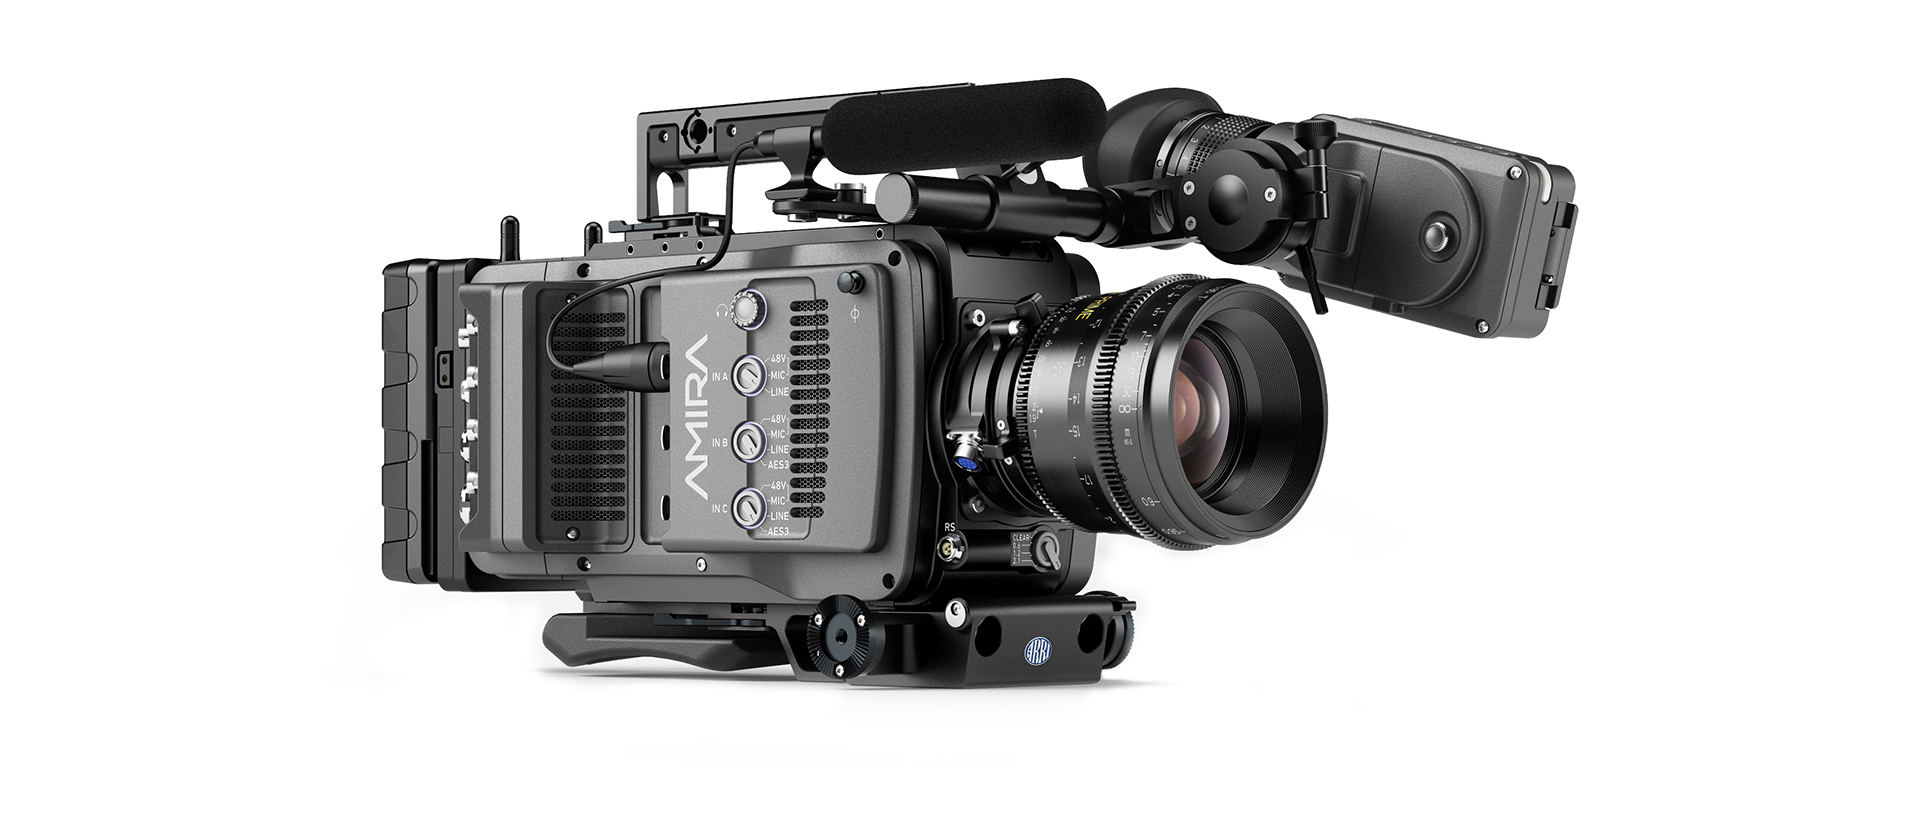
\includegraphics[width = 0.7\linewidth]{pictures/amira-product-image-data.jpg}
	\smallskip
	\caption{ARRI AMIRA \protect\footnotemark[2]}
	\label{fig:amira}
\end{figure}  
\footnotetext[2]{ \url{https://www.arri.com/resource/blob/33916/909908b1643addb99036f132d6b3582c/amira-product-image-data.jpg}}

Die AMIRA ist eine vielseitige Kamera, die für eine Einmannbedienung ausgelegt ist.
Zusätzlich ist sie mit einem Audioboard ausgestattet und aus diesem Grund bei Dokumentationsfilmen und der elektronischen Berichtserstattung gerne verwendet. Zum Beispiel wird die \ac{ARRI} AMIRA bei Sportveranstaltungen der NFL in Amerika eingesetzt. \cite{arrinewsamira} 

Für Spielfilm- und Serienproduktionen wird auch manchmal die \ac{ARRI} AMIRA eingesetzt, wodurch das breite Einsatzspektrum der Kamera noch deutlicher wird.
Als Beispiele sind hier der bayrische Eberhofer Krimi \glqq Sauerkrautkoma\grqq{} \cite{arrikrimi}, die Netflixserie \glqq The Ivory Game\grqq{} \cite{imdbivory} oder auch das Fernsehmagazin \glqq The Grand Tour\grqq{} \cite{imdbtour} zu nennen.

% Elektronische Berichtserstattung, billigste, neues marktsegement, keine andere arri kamera drinnen, live sendung bis hin zu reportage, viel bei broadcast unternehmen und sportveranstaltungen
%doku: the ivery game (netflix),  doku & aktion, super bild, und audiopoard, top gear (amazon), serien udn spielfilm (eberhofer filme), veep (us), sportveranstalungen (nfl nba) us, 2 bis 6 Kameras
%eb kamera, broadcaster, live sendung bis reportage

\subsection{Bildkette}
Unter einer Bildkette versteht man die Verarbeitungskette der Bilder vom Eingang - dem Sensorbild bis zu zum Ausgang, in unserem Fall die \ac{rec} und das \ac{sdi}.

\begin{figure}[!hbtp]
	\centering
	\includegraphics[width = \linewidth]{pictures/bildkette.png}
	\smallskip
	\caption{Schematische Bildkette}
	\label{fig:bild}
\end{figure} 

In der Abbildung~\ref{fig:bild} sieht man eine schematische Bildkette, die in dieser Arbeit zur Veranschaulichung weiter detailliert wird. 
Von der Quelle bis zur jeweiligen Senke läuft das Bild durch verschiedene Module, die für die Anpassung des Bilds sorgen. 

Direkt nach dem Sensor geht das Bild durch eine \acl{xbar}, hier wird das identische Bild in zwei Bildpfade weitergeführt. Für die \acl{rec} wird das Bild im Crop zugeschnitten, somit wird nur ein bestimmter Bildausschnitt aufgezeichnet. In dem anderen Bildpfad wird, mithilfe des Scalers, das Bild kleiner skaliert. Nachdem eine grafische Benutzeroberfläche hinzugefügt worden ist, wird das Bild am \ac{sdi} ausgegeben. Hier ist durch die Skalierung das komplette Sensorbild einschließlich der eingefügten Oberfläche zu sehen.

In dieser Arbeit wird nur das \ac{fpga}-Modul \ac{xbar} softwareseitig implementiert, da weitere Module sonst den Umfang der Arbeit überschreitet. 


\subsection{Funktionsweise}
Bevor auf das erarbeitete Konzept eingegangen wird, soll kurz auf die Funktionsweise der Kamera und die aktuelle Implementierung eingegangen werden.

Die bildverarbeitende Hauptfunktionalität liegt im \ac{fpga}. Hier werden die Module entsprechend der Bildkette angeordnet und verbunden. Durch die Software werden bei den \ac{fpga} Module Einstellungen vorgenommen.\\


Damit die Einstellungen auch zu dem Sensorbild passen, werden alle Module des \ac{fpga}s in dem \ac{geo} abgebildet. Das objektorientierte Framework führt hauptsächlich Berechnungen der Bildgrößen und Offsets durch. Nach der Änderung einer Größe in der Quelle oder Senke werden alle Module in der abgebildeten Frameworkbildkette geupdatet und entsprechend der voreingestellten Parameter werden die Größen neu berechnet. 

Nach der Änderung der Größen wird in dem entsprechenden Modul ein Flag gesetzt, welches später dafür sorgt, dass auch das Modul im \ac{fpga} aktualisiert wird. 

Beim Updaten des Modules wird an den entsprechenden Offset im \ac{fpga} die übergebenen Einstellungen geschrieben und gleichzeitig das gesetzte Flag wieder gelöscht. 

%todo umschreiben 
Damit der Zugriff auf den \ac{fpga} möglich ist, wird dieser beim Starten der Software über ein \ac{ioctl} initialisiert und anschließend kann über eine Variable im Shared Memory in allen Prozesseen darauf zugegriffen werden.

\subsection{Problematik}\label{sec:prob}
Bei der aktuellen Implementierung liegen verschiedene Probleme vor, die durch ein neues Framework eliminiert werden sollen.\\

Zum Einen muss bei den Zugriff auf ein Modul immer der \ac{fpga} gesperrt werden. Dadurch kann es passieren, dass es einen oder zwei Frames dauert, bis alle Einstellungen in der Bildkette aktuell sind.\\


Des weiteren müssen die Adressen für die \ac{fpga} Module händisch eingetragen werden. Die Fehleranfälligkeit steigt dadurch natürlich weiter, da es passieren kann, dass die Software, Einstellungen an eine Adresse schreibt, hinter der kein Modul liegt. In schlechtesten Fall werden die Register eines anderen Modules beschrieben und es kommt zum Fehlerfall in der Bildkette.\\


Auch die Länge der Register wird in der aktuellen Implementierung nicht weiter berücksichtigt. So kann es dann passieren, dass über ein Register hinweg geschrieben wird. Auch dann kommt es zum Fehlerfall in der Bildkette, da andere Einstellungen überschrieben werden. 
 
%v.4.15.9
\section{Konzept}\label{sec:konzept}
Die Probleme in der aktuellen Implementierung (siehe Kapitel~\ref{sec:prob}) sollen durch ein neues Framework behoben werden, aber die Zugriffe der Software auf den \ac{fpga} sollen auch übersichtlicher und wartbarer gestaltet werden. \\

Die Zugriffe auf den \ac{fpga} benötigen in der momentanen Implementierung immer die Adressen der Module im \ac{fpga}. Dadurch wird die Fehlersuche in diesen Teilen der Software extrem kompliziert und aufwendig. Durch das \ac{fra} sollen die Firmware Module im Kernel als Gerät angelegt werden und in der Software wird auf die \ac{fpga} Module über die entsprechenden Dateideskriptoren zugegriffen. \\


Die Geräte werden mit der Adresse, dem Name, dem Type und der Größe des dahinterstehenden Modul angelegt. Dieser Teil soll generisch generiert werden, aber aufgrund von verschiedenen Abhängigkeiten überschreitet es den Umfang der Arbeit. Deswegen werden die Geräte beim Initialisieren des Bildpfads mit den entsprechenden Parametern angelegt. \\

Das Öffnen der Dateideskriptoren erfolgt in der Software über den Namen und wird in einem Handle gespeichert. Damit ist der Zugriff ohne Adresse gewährleistet. Jeder Prozess in der Software muss seinen eigenen Dateideskriptor öffnen und verwaltet somit ein eigenes Handle. 
Im Kernel wird gewährleistet, dass nur eine maximale Anzahl von Deskriptoren geöffnet werden kann. Zusätzlich soll implementiert werden, dass es verschiedene Applikationstypen gibt. Damit kann immer nur eine echte Applikation Zugriff bekommen, allerdings sollen Debugtools immer die Möglichkeit haben zu lesen und teilweise auch zusätzlich Schreibrechte. \\

Der Zugriff auf die Module erfolgt über ein \ac{ioctl} des Treibers. Da beim Anlegen der Geräte eine Größe festgelegt wird, soll bei allen Zugriffen auf die Register überprüft werden, ob diese innerhalb der angegebenen Modulgröße liegen. Damit ist es nicht mehr möglich über ein Register hinweg zu schreiben.\\




\chapter{\acl{fra}} \label{sec:haupt}
In diesem Kapitel soll auf die  Vorgehensweise und die Implementierung des in \ref{sec:thema} vorgestellte \ac{fra} eingegangen werden. schwerpunkte.... In dieser Arbeit wird nur die \acl{xbar} softwareseitig implementiert, da es sonst den Umfang der Arbeit übersteigt.

%Aktuelle Implementierung
%Theoretische Grundlagen o.ä.
%Umsetzung

\section{Generischer Plattformtreiber} \label{sec:plat}
Um eine einwandfreie Kommunikation zwischen den Firmware Modulen im \ac{fpga} und dem Kernel zu gewährleisten, muss ein generischer Treiber erstellt werden. 


Wie in dem Kapitel~\ref{sec:plat_t} bereits erläutert, werden für die grundlegende Funktionsweise eines Treiber verschiedene Funktionen benötigt. Zunächst soll auf die Registrierungs- bzw. Aufräumfunktion des Treibers eingegangen werden.\\


Beim Laden des Treibers werden verschiedene allgemeingültige Parameter gesetzt und zusätzlich Speicherplatz allokiert. 
\begin{lstlisting}
struct afm_driver
{
	unsigned int major_id;

	uint8_t minor_list[AFM_MAX];
	spinlock_t minor_spinlock;
	struct class * class;
};
\end{lstlisting}
\captionof{code}{\label{code:afm_data}Struktur des Treibers}

Im Treiber wird beim Laden als Erstes eine Klasse erstellt, der später die einzelnen Module zugeordnet werden. Diese Klasse wird in der dem Treiber zugehörigen Struktur \textit{afm\_driver} in der Variablen \textit{class} abgespeichert. 


Da die Majornummer den Treiber kennzeichnet (siehe Kapitel~\ref{sec:mmnum_t}) wird diese in der globalen Treiberstruktur als \textit{major\_id} gespeichert. Für die Minornummer wird in der Datenstruktur eine Liste \textit{minor\_list[AFM\_MAX]} und ein zugehöriges Spinlock \textit{minor\_spinlock} initialisiert. Über die Liste wird später eine freie Nummer ausgewählt, die bei jedem Gerät individuell ist und gleichzeitig wird dadurch die Anzahl der möglichen Module auf \textit{AFM\_MAX} begrenzt. Das Spinlock sorgt bei der Auswahl der Minornummer für einen unterbrechungsfreien Vorgang, sodass keine Nummer doppelt vergeben werden kann. 


Am Ende der initialen Funktion wird der Plattformtreiber mit der \textit{platfrom\_driver} Struktur (siehe Codebeispiel~\ref{code:platform_driver}) registriert. Damit werden die initiale Funktion zum Anlegen, aber auch die Funktion zum Deinitialisieren der Geräte übergeben.


Analog wird beim Freigeben des Treibers der allokierte Speicherplatz freigegeben, der Plattformtreiber abgemeldet und die erstelle Klasse zerstört.\\


Beim Anlegen einer Instanz vom Treiber wird die \textit{.probe} Funktion aufgerufen und zusätzlich wird der Modultyp und Name in einer \textit{arri\_fra\_mod\_config} Struktur zur Verfügung gestellt.
%todo aussotieren
\begin{lstlisting}
struct afm_device 
{
	struct arri_fra_mod_config *mod_config;
	
	struct class *class;
	struct cdev cdev;
	unsigned int minor_id;
	struct platform_device *pdev;
	struct resource *res;
	u8 __iomem *base;
	
	struct afm_file fdev[AFM_FILE_MAX];
	spinlock_t open_spinlock;
	%atomic_t use_count;
	
	#define AFM_NOLOGGING   ((uint32_t)0U)
	#define AFM_LOGGING     ((uint32_t)1U)
	uint32_t has_logging;
};
\end{lstlisting}
\captionof{code}{\label{code:afm_device}Auszug aus der Struktur einer Instanz}

In der initialen Funktion der Instanz wird diese Struktur genutzt um spezifische Einstellungen für jede einzelne Instanz festgelegt und in einer entsprechenden Datenstruktur (siehe Codebeispiel~\ref{code:afm_device}) gespeichert. 


Der einzige Übergabeparameter der Probefunktion ist die Struktur des \textit{platform\_device}, diese wird in dem Zeiger \textit{*pdev} gespeichert. Auch die, beim Laden des Treibers, angelegte Klasse wird ohne weitere Änderungen unter \textit{*class} abgelegt. 

Aus der Liste der Minornummern (siehe Codebeispiel~\ref{code:afm_data}) wird nach dem Sperren des zugehörigen Spinlocks eine freie Nummer ausgewählt und als \textit{minor\_id}, sowie auf verwendet gesetzt. 

Anschließend wird mit Hilfe der Majornummer und der Minornummer ein Device erstellt und als \textit{cdev} gespeichert. 

%todo vorteile statischer speicher
Damit das Öffnen der Devices auf eine bestimmte Anzahl limitiert ist, wird beim Initialisieren der Instanz ein Array der \textit{afm\_file} Struktur angelegt. Gleichzeitig wird der Speicherplatz statisch zur Kompilierzeit reserviert. Durch den Spinlock \textit{open\_spinlock} wird später dafür gesorgt, dass die Auswahl nicht unterbrochen und somit verfälscht wird.

%todo base/res

\section{Konzeptionierung der \acl{ioctl}s}\label{sec:ioctl}
%todo zu oft ioctl
%über ioctl zugriff auf das geöffnete Device
%Auf die ioctl eingehen und die Überlegungen hinter diesen
%hello, logging/unlogging?, get id, get reg, get reg bitmask, get reg block, set reg, set reg bitmask, set reg block, 
In dem Abschnitt soll auf die Konzeptionierung der \ac{ioctl}s eingegangen werden. Wie in Kapitel~\ref{sec:ioctl_t} erläutert werden \ac{ioctl}s benötigt um zwischen Kernel und Userspace Daten auszutauschen. Da der Großteil der Software im Userspace läuft, aber der Treiber im Kernel, wird der hauptsächliche Zugriff auf die Geräte über \ac{ioctl}s geregelt.\\


Als Erstes ist eine Anmeldung der Anwendung bei dem Gerät notwendig. Um die Eindeutigkeit zu garantieren wird hier die \ac{pid} übergeben. Allerdings wird auch der Prozessname benötigt, damit eine schnelle Nachvollziehbarkeit vorhanden ist. Wie in Kapitel~\ref{sec:konzept} erläutert, soll die Unterscheidung zwischen Standardapplikation und Debugtool möglich sein. Aus diesem Grund wird bei der Anmeldung zusätzlich zur \ac{pid} und dem Prozessnamen auch der Typ der Applikation übergeben. 
%todo satz hier oder wo anders?
Ohne die Ausführung von dem \textit{ARRI\_FRA\_MOD\_HELLO} \ac{ioctl} bleibt der weitere Zugriff auf das Gerät über \ac{ioctl}s verwehrt.\\

Die Protokollierung der Zugriffe auf ein Gerät ist ein notwendiger Bestandteil. Dadurch soll vor allem im Fehlerfall, die Suche erleichtert werden. Aufgrund der Zugriffe durch verschiedene Prozesse besteht ohne Protokollierung kein einheitlicher Überblick über diese.
In dem Zusammenhang werden zwei \ac{ioctl}s angelegt. Dabei ist \textit{ARRI\_FRA\_MOD\_LOGGING} zum Aktivieren der Protokollierung zuständig und analog wird diese durch \textit{ARRI\_FRA\_MOD\_NOLOGGING} deaktiviert. \\

Beim Anlegen des Geräts werden der Gerätetyp und der Name abgelegt. Im Userspace soll nach dem Öffnen des Geräts auf diese Informationen zugegriffen werden. Dafür wird ein eigenes \ac{ioctl} benötigt, welches den Typ und Namen aus der Instanzstruktur (siehe Codebeispiel~\ref{code:afm_device}) zurück gibt.\\

Die essenziellen Funktionen des Treibers sind das Setzen bzw. Auslesen von Register. Basierend auf den in der aktuellen Implementierung genutzten Funktionen und den entsprechenden Registerzugriffen, gibt es bis zu drei verschiedene Arten. Jede soll durch ein eigenes \ac{ioctl} abgebildet werden, da so die spätere Verwendung vereinfacht wird.  


Die Größe eines Registers ist auf 4 Byte normiert. Damit werden zum einfachen Setzen eines Registers lediglich zwei Parameter benötigt. Zum Einen die Stelle des Registers im Gerät(auch Registernummer) und zum anderen der Inhalt. 
Allerdings besteht auch die Notwendigkeit einzelne Bits oder mehrere hintereinander liegende Register über einen Aufruf zu setzen. Für beide gibt es ein gesondertes \ac{ioctl}. Zum Setzen von einzelnen Bits wird zusätzlich zu den beiden oben genannten Parametern noch eine Bitmaske übergeben. Mithilfe der Bitmaske werden im Register erst die entsprechenden Bits gelöscht und danach gesetzt. Dadurch ist es nicht notwendig erst über ein \ac{ioctl} das entsprechende Register auszulesen, anschließend im Userspace zu verändern und dann, wieder über ein \ac{ioctl}, in das gleiche Register zu setzen.
Der zweite Sonderfall benötigt andere Übergabeparameter als das einfache Setzen. Zusätzlich zu der Registernummer wird hier eine Registeranzahl gebraucht. Des Weiteren muss der Inhalt der Register in einem Array mit der Größe der Anzahl übergeben werden. Damit kann dann der Reihe nach jedes Register einzeln mit dem entsprechenden Inhalt beschrieben werden.


Das Auslesen der Register erfolgt nahezu analog zu dem Setzen. Der Parameter für den Registerinhalt wird hier allerdings über das \ac{ioctl} gefüllt und dann zurück in den Userspace übergeben. 
Register über eine Bitmaske auszulesen würde keine weiteren Vorteile gegenüber den Auslesen des ganzen Registers bieten. Aus diesem Grund wird es nicht implementiert.  
Damit man einen ganzen Block an Registern zurück lesen kann, muss durch das übergeben eines leeren Arrays mit der richtigen Größe der Speicherbereich zu Verfügung gestellt werden.\\

Dadurch sind die wichtigsten \ac{ioctl}s erläutert, die notwendig sind um die Grundfunktionen des Geräte abzudecken und zusätzlich eine triviale Debug Möglichkeit bieten.

\section{Implementierung im Kernel}\label{sec:kernel}
% Anlegen der Devices (arrifpga), Über Ioctl im Arri fpga treiber, öffnen und schließen des device, im eigenen Verzeichnis
% ioctl implementierung im kernel, was steht dahinter, wie funktioniert es, auszüge
Im Kernel gibt es zwei verschiedene Stellen, an welchen der Code implementiert ist. Zum einen muss der \ac{fpga} Treiber entsprechend erweitert werden, damit die Geräte unter Linux angelegt werden und zum anderen der \ac{fra} Treiber, um die angelegten Geräte zu Öffnen bzw. zu Schließen. \\

Zur besseren Übersichtlichkeit wurde sich für zwei Nameskonventionen entschieden. Strukturen und Funktionen, die mit \textit{arri\_fra\_mod} beginnen, werden außerhalb des \ac{fra} Treibers benötigt bzw. angelegt. Mit diesem Prefix werden die Namen recht lang, aus diesem Grund wird treiberintern auf den nicht so aussagekräftigen Prefix \textit{afm} abgekürzt.



%todo _static_assert mit aufnehmen

\subsection{Anlegen der Geräte}
%im fpga treiber
Der Zugriff der Software auf die \ac{fpga}-Module soll über Geräte stattfinden. Durch die unterschiedlichen Funktionalitäten der Module, wie in Kapitel~\ref{sec:bildkette} erläutert, werden diese Geräte als Kindgeräte vom \ac{fpga} angelegt, d.h. kernelseitig wird dieser Bestandteil im vorhandenen \ac{fpga} Treiber implementiert. 

\begin{lstlisting}
struct arri_fra_mod_init 
{
	#define ARRIFPGA_FRA_MAX_NAME   ((uint32_t)50)
	char type[ARRIFPGA_FRA_MAX_NAME];
	char name[ARRIFPGA_FRA_MAX_NAME];
	uint32_t offset;
	/* register size in bytes */
	uint32_t size;
};
\end{lstlisting}
\captionof{code}{\label{code:arri_fra_mod_init} Struktur zum Initialisieren des Geräts}

Über ein \ac{ioctl}, mit der obigen Struktur als Übergabeparameter, wird das Gerät angelegt. 


Als Erstes wird hier Speicherplatz für die drei Strukturen \textit{resource}, \textit{mfd\_cell} und \textit{arri\_fra\_mod\_config} allokiert. Mithilfe dieser am Ende der Funktion, die durch das \ac{ioctl} aufgerufen wird, das \ac{mfd} angelegt.


In der \textit{resource} Struktur (siehe Codebeispiel~\ref{code:res}) wird der Speicherbereich des \ac{fpga}-Modules abgebildet. Für die Variable \textit{start} wird auf den bereits allokierten \ac{fpga} Bereich noch der im \textit{arri\_fra\_mod\_init} übergebene \textit{offset} aufaddiert. Entsprechend ist wird für den \textit{end} Wert noch die \textit{size} addiert und zusätzlich eins abgezogen, da alles null basiert ist. Durch den Parameter \textit{flags} wird die Ressource als Speicherbereich festgelegt und als \textit{parent} wird die Ressource des gesamten \ac{fpga}s angegeben.


Als Nächstes wird die \textit{mfd\_cell} Struktur (siehe Codebeispiel~\ref{code:mfd_cell}) gefüllt. Hier wird die Variable \textit{id} auf eine globale Variable gesetzt, die bei jedem Funktionsaufruf um eins erhöht wird. \textit{num\_resources} wird auf eins gesetzt, da es für jedes Gerät nur eine Ressource gibt. Entsprechend wird in  \textit{resources} der aktuelle Zeiger der Ressource übergeben. Analog wird in \textit{platform\_data} der Zeiger auf die \textit{arri\_fra\_mod\_config} Struktur und in \textit{pdata\_size} die Größe der Struktur abgelegt.
Durch die \textit{arri\_fra\_mod\_config} wird der Gerätename und -typ an den Treiber übergeben.


Über die im Codebeispiel~\ref{code:mfd} aufgezeigt Funktionsdeklaration wird das Gerät angelegt. Dadurch wird die \textit{.probe} Funktion des Plattformtreibers ausgeführt und das erfolgreich angelegte Gerät ist auf der Kamera unter \textit{/dev/fra} zu finden.


\subsection{Öffnen und Schließen der Geräte}
%kernelseitige  implementierung im Treiber
Um später im Userspace auf die Geräte zuzugreifen und um initiale Einstellungen vorzunehmen, muss eine \textit{open} Methode implementiert werden. Im Umkehrschluss werden die Einstellungen durch die \textit{release} Funktion rückgängig gemacht. \cite[Seite 58f.]{corbet2005linux} \\

Die Anzahl von offenen Geräten ist durch die Speicherallokierung in der Struktur \textit{afm\_device} (siehe Codebeispiel~\ref{code:afm_device}) auf \textit{AFM\_FILE\_MAX} (hier: 4) begrenzt. Die geöffnete Instanz eines Geräts wird in der Struktur \textit{afm\_file} abgelegt.

\begin{lstlisting}
struct afm_file {  
#define AFM_FREE    ((uint8_t)0U)
#define AFM_USED    ((uint8_t)1U)
	uint8_t in_use;
	struct afm_device *dev;
	int minor;
	char name[ARRI_FRA_MOD_MAX_NAME];
	uint32_t type;
	uint32_t pid;
#define AFM_UNLOCK  ((uint32_t)0U)
#define AFM_LOCK    ((uint32_t)1U)
	uint32_t has_lock;
	struct file *file;
};
\end{lstlisting}
\captionof{code}{\label{code:afm_file} Struktur zum Ablegen des Geräts}
%todo caption umbenennen

Beim Öffnen eines Geräts wird, nachdem das entsprechende Spinlock (\textit{open\_spinlock}) gesperrt wurde, nach einem freien Gerät zum Öffnen gesucht. Hierzu wird über eine for-Schleife iteriert, bis die maximale Anzahl erreicht ist. In jedem Durchgang wird die Variable \textit{in\_use} überprüft, entsprechend dem Define kann dann festgestellt werden, ob es noch möglich ist ein Gerät zu öffnen. Wurde eine freie Stelle gefunden, wird der Parameter auf \textit{AFM\_USED} gesetzt und das Spinlock wieder freigegeben.
Wenn die maximale Anzahl erreicht ist, wird eine Fehlermeldung ausgegeben und ein Fehlercode zurückgehen.
Die Variable \textit{dev} wird auf das geöffnete Gerät gesetzt, analog wird \textit{minor} auf die verwendete Minornummer und \textit{file} auf die, in der \textit{open} Methode, übergebene Datei gesetzt. 
\textit{has\_lock} wird beim Öffnen des Geräts initial freigegeben. Die anderen Parameter beschreiben den Prozess, welcher das Gerät öffnet und werden durch ein \ac{ioctl} entsprechend beschrieben.\\

Analog werden in der \textit{release} Funktion, die Inhalte aus \textit{file} und \textit{dev} auf \textit{NULL} gesetzt. Dadurch ist keine Zuordnung mehr möglich und durch das Freigeben der Variable \textit{in\_use} kann beim nächsten Öffnen der Eintrag im Array überschrieben werden.


\section{Implementierung im Userspace}\label{sec:user}
%öffnen und schließen der Devices, testprogramm, über namen, (überlegungen zu Test und Backend entscheidung) -> oder in ioctl implem.
%Implementierung der ioctls im Userspace, zweites testprogramm, backend!
%testprogramm
%xbar
%überlegungen zum testen, backend entscheidung
Der Zugriff auf die \ac{fra} Module im Userspace ist in zwei Ebenen gekapselt. Die untere Stufe besteht aus verschiedenen backendspezifischen Funktionen. Entsprechend sind in der anderen Ebene erweiterte Wrapper Funktionen zu finden. Hier werden verschiedene Überprüfungen durchgeführt, damit kein fehlerhafter Zugriff stattfindet. Des Weiteren wird im Wrapper entsprechend dem Backendtyp, die unterliegende Funktion ausgewählt. Damit es den Umfang der Arbeit nicht übersteigt, wird nur das Kernelbackend implementiert. Dies wird benötigt um über die, im Kernel implementierten, \ac{ioctl}s auf die \ac{fpga} Module zuzugreifen. 

Durch die gekapselten Ebenen ist eine Erweiterung um neue Backendtypen einfach gestaltet.  Insbesondere über ein Testbackend sollen Unittest zu den verschiedenen Modulen möglich sein, damit können Fehler frühzeitig erkannt, eingegrenzt und behoben werden. 
Durch die Kapselung ist die Wartbarkeit erhöht worden. Dadurch müssen bei Änderungen im Kernelzugriff, nur im Backendcode die entsprechenden Stellen geändert werden.\\

\subsection{\ac{fra} Bibliothek}
%fra_handle
%Wrapper
%fra_init
%grundfunktionen
Neben den Wrapper Funktionen wird in der \ac{fra} Bibliothek auch eine Struktur zum Abspeichern der wichtigen Parameter der \ac{fra} Module im Userspace bereitgestellt.

\begin{lstlisting}
struct fra_handle
{
	int dev;
	char dev_type[FRA_MAX_NAME];
	char dev_name[FRA_MAX_NAME];
	uint32_t type_id;
	const struct fra_backend_funcs *backend_funcs;
};
\end{lstlisting}
\captionof{code}{\label{code:fra_handle} Struktur zum Abspeichern wichtiger Parameter}

%todo file discrioter deutsch?
Der erste und wichtigste Parameter in der Struktur ist der File Descriptor. \textit{dev} Hierüber kann nach dem Öffnen des Geräts weiterhin auf dieses zugegriffen werden. Die restlichen Parameter werden beim initiieren des Geräts gesetzt. \textit{dev\_type} und \textit{dev\_name} geben den Modultyp und den Namen an. Für spätere Überprüfungen wird gibt es für jeden Modultyp noch ein Define, dieses wird in der Variablen \textit{type\_id} abgelegt. In der \textit{fra\_backend\_funcs} Struktur sind Prototypen aller backendspezifischen Funktionen abgelegt.\\

Das Öffnen eines Geräts ist nur über die \textit{fra\_init} Funktion möglich. Da neben dem Öffnen auch eine Anmeldung bei dem Gerät stattfinden muss (siehe Kapitel~\ref{sec:ioctl}), wird dies über einen Funktionsaufruf abgedeckt. 


Der initiialen Funktion wird auch ein Backendtyp übergeben und anhand von diesem die Funktionsstrukur im \textit{fra\_handle} gesetzt. Anschließend wird das Gerät geöffnet und danach meldet sich der Prozess direkt an. Hierzu werden jeweils die entsprechenden Wrapper Funktionen aufgerufen um die Funktionalität bei allen Backendtypen zu garantieren. Zum Bestimmen von \textit{dev\_type} und \textit{dev\_name} wird auch über eine Wrapper Funktion, diese Parameter vom Gerät geholt und entsprechend im \textit{fra\_handle} gesetzt. Durch das Iterieren über eine \textit{fra\_type\_list} mit Name, ID und Größe und dem Vergleichen der Strings in Name und dem \textit{dev\_name} wird die Variable \textit{type\_id} gesetzt.\\

Die Grundstruktur der Wrapper Funktionen ist für alle identisch, deshalb wird im folgenden beispielhaft die \textit{fra\_set\_reg} näher betrachtet. Grundsätzlich gibt es für jedes konzeptioniertes \ac{ioctl} im Kernel eine Wrapperfunktion, lediglich das Logging ist in einer Funktion zusammengefasst. 

Zu Beginn einer jeden Methode wird über ein Makro verschiedene Überprüfungen durchgeführt. 

\begin{lstlisting}
#define FRA_CHECK_HANDLE(p_handle)         \
	if (p_handle == NULL)                    \
	{                                        \
		return ERRVALUE_INVALID_PARAMETER;     \
	}                                        \
	if (p_handle->dev == -1)                 \
	{                                        \
		return ERRVALUE_DEVICE_NOT_OPEN;       \
	}                                        \
	if (p_handle->backend_funcs == NULL)     \
	{                                        \
		return ERRVALUE_NOT_INITIALIZED;       \
	}  
\end{lstlisting}
\captionof{code}{\label{code:fra_check_handle} Makro zum Überprüfen des Handles}

Ohne ein gültiges Handle machen alle nachfolgenden Aufrufe keinen Sinn, da alles basierend auf diesem Handle erfolgt. Aus diesem Grund wird dies in Zeile 2 als erstes überprüft. Über den File Descriptor kann man herausfinden, ob das Gerät schon geöffnet wird. Hier wird beim initiieren der Struktur \textit{dev} auf -1 gesetzt. Als letztes wird noch überprüft, ob ein Zeiger auf die \textit{fra\_backend\_funcs} Struktur übergeben wurde. Die Funktion, in welcher das Makro aufgerufen wird gibt entsprechende, intern definierte Fehlermeldungen zurück um die Fehlersuche zu erleichtern.\\

In der Funktionssignatur ist immer das \textit{fra\_handle} und die \textit{transid} angeben. Durch das Handle werden alle notwendigen Informationen zum Zugriff auf das Gerät übergeben und die Transaktionsidentifikation ist in der Signatur implementiert, damit bei einer späteren Erweiterung nicht alle Aufrufe geändert werden müssen. Aktuell wird sie lediglich bis zum Ende durchgereicht und nicht weiter beachtet. 

\begin{lstlisting}
/*  fra_set_reg(handle, transid, num, reg)
 *      sets a register at num
 */
int32_t fra_set_reg(struct fra_handle const *handle,
					const uint32_t transid,
					const uint32_t num, 
					uint32_t reg)
{
	FRA_CHECK_HANDLE(handle);

	if (!handle->backend_funcs->fra_set_reg) return ERRVALUE_FUNCTION_NOT_AVAILABLE;
	return handle->backend_funcs->fra_set_reg(handle, transid, num, reg);
} /* fra_set_reg () */
\end{lstlisting}
\captionof{code}{\label{code:fra_set_reg} Funktion zum Setzen eines Registers}

Das Makro in Zeile 9 ist im Codeausschnitt~\ref{code:fra_check_handle} näher ausgeführt. 
Durch die if - Bedingung in Zeile 11 wird überprüft, ob für das ausgewählte Backend die entsprechende Funktion implementiert ist. Damit wird vermieden, dass beim Aufrufen der Funktion auf \textit{NULL} zugegriffen wird und somit beim laufenden Programm ein Fehler auftritt. Der Rückgabewert in der Funktion in der \ac{fra} Bibliothek entspricht entweder einem entsprechenden Fehlerwert bzw. dem Rückgabewert der Backendfunktion. 


\subsection{Kernelbackend}
Da die Wrapper lediglich alle benötigte Übergabeparameter an die Backendfunktionen weiterreichen, haben diese eine identische Funktionssignatur. 
Die einzelnen Funktionen unterscheiden sich im Kernelbackend nur durch die aufgerufenen \ac{ioctl}s und entsprechenden den übergebenden Strukturen dazu. Beispielhaft soll hier wieder die Funktion zum setzen eines Registers betrachtet werden. 


Hier finden keine weiteren Überprüfungen statt, da dies bereits eine Ebene höher geschehen ist. Nach dem Füllen der Übergabestruktur wird das \ac{ioctl} aufgerufen und anschließend auf Fehler überprüft. 
Im Fehlerfall wird eine Meldung ausgegeben und der Fehlerwert zurückgegeben. 

\begin{lstlisting}
int32_t fra_kernel_set_reg(struct fra_handle const *handle, const uint32_t transid, const uint32_t num, uint32_t reg)
{
	(void) transid;
	int32_t retval = ERRVALUE_SUCCESS;
	int32_t err;
	struct arri_fra_mod_reg frareg;
	
	frareg.num = num;
	frareg.reg = reg;
	err = ioctl(handle->dev, ARRI_FRA_MOD_SET_REG, &frareg);
	if (err < 0)
	{
		error_msg(EH_ERROR, "%s: FRA IOCTL failed. (%u)", handle->dev_name, err);
		retval = ERRVALUE_IOCTL_FAILED;
	}  
	return retval;
} /* fra_kernel_set_reg () */
\end{lstlisting}
\captionof{code}{\label{code:fra_kernel_set_reg} Funktion im Kernelbackend zum Setzen eines Registers}


\section{Einbindung ins \acl{geo}}\label{sec:soft}
%anlegen der Devices in der software, öffnen der devices über den module_idx und abspeichern im entsprechenden handdle, abändern der funktionen von fpga zugriff auf fra zugriff und hw update lediglich über den module_idx des geo module möglich, da über den identischen namen geöffnet wurde und handle unter dem idx gespeichert ist, umstellen des hw update auf die neuen Funktionen
%Bild?
Um das \ac{fra} vollständig in der Kamerasoftware zum Implementieren müssen die Geräte angelegt, geöffnet, geupdatet und auch wieder geschlossen werden. \\


Angelegt werden die Geräte aktuell beim Laden des \ac{fpga}s. An dieser Stelle ist bekannt, welche Firmware geladen wurde und entsprechend kann über eine Struktur bestimmt werden, ob und an welcher Stelle ein bestimmtes Modul vorhanden ist. Mit einem vorgegebenen Namen und Modultyp werden so die Geräte im Kernel angelegt. Anschließend kann in der kompletten Kamerasoftware davon ausgegangen werden, dass, sofern kein Fehler aufgetreten ist, die Geräte verfügbar sind.  \\


Beim initialen Hardwareupdate durch das \ac{geo} werden für alle vorhandenen, in diesem Framework abgebildeten Module ein Gerät geöffnet und entsprechend dem Modulindex in ein \textit{fra\_handle} abgelegt.\\


Damit die Module geupdatet werden können, müssen die vorhandenen Funktionen, welche direkt an die Offsets im \ac{fpga} schreiben geändert werden. Im Rahmen dieser Arbeit wird lediglich die \ac{xbar} näher betrachtet, aber andere Module müssen analog abgeändert werden.

In den Hardwarefunktionen des \ac{geo} werden für die \ac{xbar} die Konfiguration der Ein- und Ausgänge aus dem Framework gezogen und anschließend die \textit{fra\_xbar} Funktion aufgerufen, welche die vorherige \textit{fpga\_xbar} Funktion ersetzt und für die richtige Einstellung in der Hardware zuständig ist.


\begin{lstlisting}
int32_t fra_xbar(struct fra_handle const *handle, const uint32_t transid, const uint32_t setting)
{
	int32_t retval = ERRVALUE_SUCCESS;
	uint32_t num, reg;
	
	FRA_CHECK_HANDLE_TYPE(handle, FRA_MOD_TYPE_XBAR);
	
	num = AVALONVIDEO_CROSSBAR_MXN_ENABLE_OUTPUT_REG;
	reg = setting;
	
	retval = fra_set_reg(handle, transid, num, reg);  
	
	return retval;
}
\end{lstlisting}
\captionof{code}{\label{code:fra_xbar} Funktion zum Setzen der \ac{xbar}}

Die Funktion im Codeausschnitt~\ref{code:fra_xbar} verbindet Ein- und Ausgänge in der \ac{xbar} entsprechend dem übergebenen \textit{setting}. Durch das Makro \textit{FRA\_CHECK\_HANDLE\_TYPE} wird überprüft, ob das Gerät im \textit{handle} eine \ac{xbar} ist. Wenn dies nicht der Fall ist, wird ein entsprechender Fehlercode zurückgegeben und die Funktion ist beendet. 
Anschließend werden die Übergabeparameter für \textit{fra\_set\_reg} befüllt und die Funktion aufgerufen. 








%todo kapitel ändern!
\chapter{Frameworktest} \label{sec:test}
% testbackend muss noch geschrieben werden
% überlegungen zum testen aufschreiben 
Überprüfen der Funktionalität von den einzelnen Bestandteilen außerhalb der eigentlichen Anwendung gehört zum Entwickeln von Software dazu. %todo Quelle
Zusätzlich werden auch Tools zum Testen und Debuggen auf der Zielentwicklungsumgebung benötigt. 
In diesem Kapitel sollen beide Varianten näher betrachtet werden.

%todo titel!!
%todo glossar unittest
%todo bild
\section{Plattformunabhängige Tests}
Zunächst sollen auf die Tests eingegangen werden, die unabhängig von der Entwicklungsumgebung durchgeführt werden können. 
Damit dies möglich ist, muss die Struktur des \ac{fra} Handle angepasst sowie ein entsprechendes Testbackend implementiert werden. Anschließend können verschiedene Tests erstellt werden, wobei die Unittest im Vordergrund stehen. Hier durch kann die \ac{fra} Middleware und Bibliothek unabhängig von der Software getestet und bei Änderungen überprüft werden, ob die beiden Teile korrekt arbeiten.

\begin{figure}[!hbtp]
	\centering
	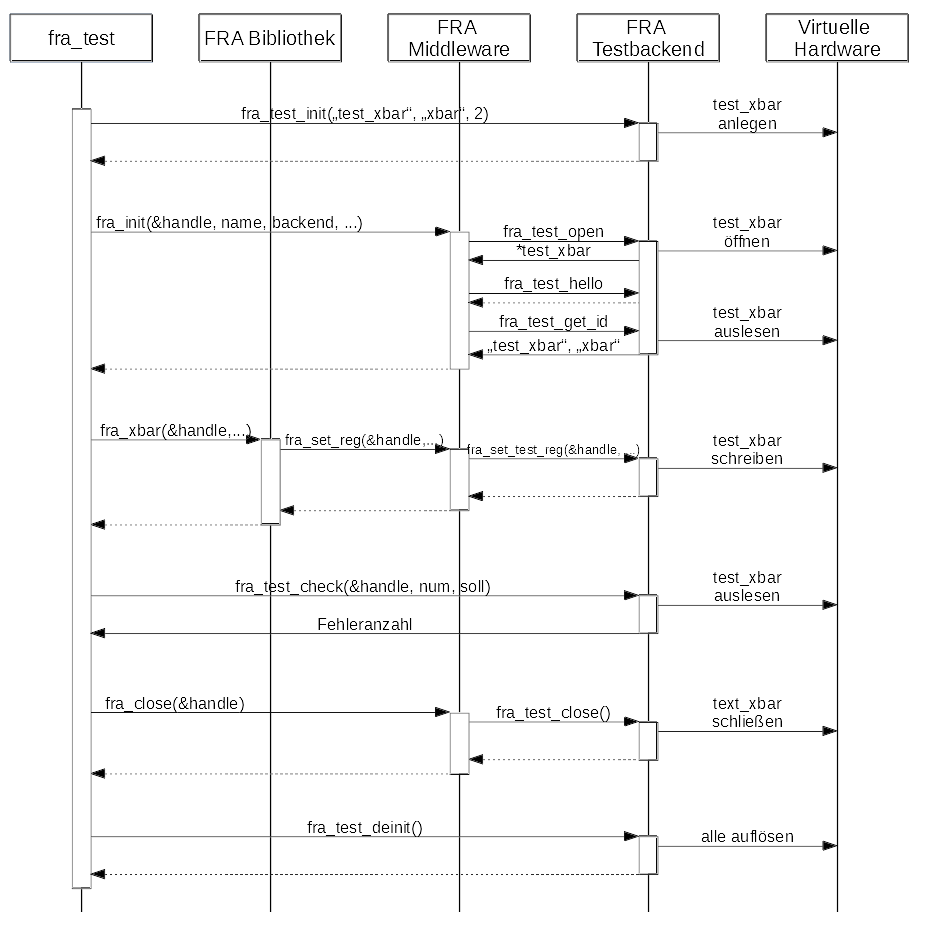
\includegraphics[width = \linewidth]{pictures/2019-11-28-testbackend.png}
	\smallskip
	\caption{Beispielhaftes Sequenzdiagramm zum Unittest}
	\label{fig:testbackend}
\end{figure} 


\begin{lstfloat}
\begin{lstlisting}
struct fra_test_mod
{
	char type[FRA_MAX_NAME];
	char name[FRA_MAX_NAME];
	uint32_t size;
	uint32_t *reg;
};
\end{lstlisting}
\captionof{code}{\label{code:fra_test_mod} Struktur zum Abbilden der vituellen Hardware}
\end{lstfloat}

Durch das Anlegen eines Geräts im Kernelbackend können alle benötigten Informationen und Register über dieses Gerät abgefragt und gesetzt werden. Da das Testbackend unabhängig laufen soll, ist das Anlegen von Geräten so nicht möglich. Um eine ähnliche Funktionalität wie im Kernel zu haben, wird das Modul über die \textit{fra\_mod\_test} Struktur abgebildet. Hier werden alle notwendigen Informationen angelegt und auch entsprechende Register abgebildet, damit man diese beschreiben und auch auslesen kann.
Die \textit{fra\_mod\_test} Struktur wird als statisches Array im Testbackend angelegt und bildet so die virtuelle Hardware für das Testprogramm. Dadurch ist das Überprüfen der Register später möglich und auch eine maximale Anzahl der Module ist vorgegeben. 


Damit die virtuelle Hardware richtig initialisiert wird, muss für die Register entsprechender Speicherplatz allokiert, aber auch die restlichen Parameter gesetzt werden. Analog dazu muss der Speicherbereich der Register beim Beenden des Programms wieder freigegeben werden. Dafür gibt es im Testbackend zusätzliche Funktionen, die sich um das initialisieren und deinitialisieren kümmern.\\

 
Beim Starten des Test wird der \textit{fra\_test\_init} Funktion drei Parameter übergeben. Zum Einen wird der Name sowie der Typ des Moduls und zum Anderen wird die Größe des Registers in die Funktion gereicht. Ist die maximale Anzahl der Module noch nicht überschritten, wird mithilfe der Größe ein Registerblock allokiert. Anschließend wird die \textit{fra\_mod\_test} Struktur mit allen vier Parametern gefüllt und eine statische Variable \textit{mod\_count} erhöht.

Wenn der Test am Ende angelangt ist, werden in der \textit{fra\_test\_deinit} Funktion mithilfe der Variablen \textit{mod\_count} alle allokierten virtuellen Geräte wieder freigegeben.\\


Zum Öffnen eines Moduls im Testbackend wird analog zum Kernelbackend die Funktion \textit{fra\_init} aufgerufen. Hier wird allerdings ein anderer Backendtyp übergeben und somit in den Wrapperfunktionen entsprechend ins Testbackend weitergeleitet. 
Die Funktionalität der einzelnen Backendfunktionen sind, im Vergleich zum Kernelbackend, vereinfacht worden und kommen entsprechend ohne \ac{ioctl}s aus. Das Setzen und Lesen der Register erfolgt nun über die \textit{fra\_mod\_test} Struktur im Handle. Diese wird bei der \textit{fra\_test\_open} Funktion als Zeiger auf die entsprechende Stelle im statischen \textit{fra\_mod\_test} Array beschrieben. Die richtige Stelle wird über einen Vergleich mit dem Modulname gefunden.\\



Damit überprüft werden kann, ob die Register richtig beschrieben bzw. ausgelesen worden sind, gibt es zwei Funktionen. Diese sind, wie die \textit{fra\_test\_init} und \textit{fra\_test\_deinit} Funktion, im Testbackend, aber werden ohne Wrapperfunktion aufgerufen, da sie spezifisch sind und lediglich beim Testen genötigt werden.
Der \textit{fra\_test\_check} Funktion werden neben dem Handle noch die Registernummer und der Sollwert des Registers übergeben. Über den Namen wird die Zuordnung des Handles zu der virtuellen Hardware gemacht und anschließend der Registerwert mit dem Sollwert verglichen. Bei einem fehlerhaften Wert wird eine Fehlermeldung ausgegeben und der Rückgabewert \textit{1}.
Durch eine weitere Funktion (\textit{fra\_test\_check\_all}) kann das gesamte Register überprüft. Allerdings muss hier neben dem Handle noch ein Array der Registergröße übergeben werden. In diesem Array müssen die Sollwerte in richtiger Reihenfolge gespeichert sein. Anschließend wird für jede einzelne Registerstelle die \textit{fra\_test\_check} Funktion aufgerufen. Am Ende wird die Gesamtanzahl der Fehler zurückgegeben, welche im Test ausgewertet wird.\\


Im Unittest wird zunächst die virtuelle Hardware angelegt und geöffnet, anschließend werden modulspezifische Funktionen aufgerufen und direkt danach der Check durchgeführt (siehe Abbildung~\ref{fig:testbackend}). Dadurch kann die Funktionalität der einzelnen Module überprüft und im Fehlerfall direkt gehandelt werden. Vor allem bei Änderungen an der \ac{fra} Bibliothek können so vor der Inbetriebnahme auf der Kamera Fehler gefunden und ausgebessert werden.


\section{Tools für die Entwicklungsumgebung}
Unabhängig von der Funktionstests des vorherigen Kapitels sollten dem Entwickler kleine Programme zur Verfügung gestellt werden, mit denen man für Testprogramme oder zur Fehlersuche im laufenden Betrieb ein Gerät anlegen oder das Logging aktivieren kann.\\


Besonders für die Kalibrierung der Kamera ist es notwendig ein Gerät über die Kommandozeile anzulegen, da es hier keinen Codeteil gibt in welchem man das Anlegen integrieren könnte. Dadurch das die benötigten Geräte vor dem Starten der Kalibiersoftware angelegt werden, können in der Software über die Funktionen der \ac{fra} Bibliothek die Geräte geöffnet und auf diese zugegriffen werden.


Beim Ausführen des Programms \textit{fra\_create\_device} werden in der Kommandozeile über Optionen die benötigten Parameter übergeben. Hier gibt es neben dem Namen, dem Typ, der Adresse und der Größe auch die Möglichkeit eine Hilfe auszugeben, in welcher genauer erläutert wird, wie das Programm zu nutzen ist. 
Nach dem Ausführen des Programms werden die programminternen Parameter mithilfe der Optionen gefüllt und nach der Überprüfung auf Dateninkonsistenz wird das entsprechende Gerät angelegt. 
Danach ist dieses Gerät in Linux unter \textit{dev/fra} zu finden und weitere Programme oder Testtools können darauf zugreifen.\\

Ein weiteres nützliches Tool für die Entwicklungsarbeit ist das \textit{fra\_set\_logging}. Da das Logging standardmäßig deaktiviert ist, muss dieses bei Bedarf aktiviert werden. Damit der Entwickler nicht im entsprechenden Code die Aktivierung vornehmen und neu kompilieren muss, welches recht zeitaufwendig ist, wird durch das Testtool ein entsprechendes Werkzeug bereitgestellt. Durch das Programm kann im laufenden Betrieb der Kamera die Protokollierung eines Geräts aktiviert oder deaktiviert werden.


Hier werden beim Starten des Programms auf der Kommandozeile entsprechend den Optionen der Name des Geräts und ein Setparameter übergeben. 
Über den Setparameter wird entschieden, ob das Logging aktiviert (\textit{set=1}) oder deaktiviert (\textit{set=0}) werden soll. Anschließend wird das Gerät über den Namen geöffnet und über das entsprechende \ac{ioctl} wird des Logging gesetzt. Nach dem Schließen des Geräts wird das Programm beendet. \\


Beide Tools sind für den Einsatz auf der Entwicklungsumgebung gedacht und sollen Entwicklern und Testern vor allem die Fehlersuche auf der Kamera erleichtern. Bei Bedarf können die Programme einfach erweitert werden oder weitere Tools in Anlehnung an die Codestruktur geschrieben werden. 
\chapter{Fazit und Ausblick}
% Transaktionsids
% Bild Anton
%Die Abhängigkeit von einem händisch eingetragenen Offset ist so immer noch vorhanden!!!
% weitere vorgehensweise, weitere module, speicherbereiche, arbeitsaufwand: ca halbes jahr


\section{Zusammenfassung der Ergebnisse}
%letzes framework zum umstrukturieren der software, 
% abstraktion zur hardware, kein direkter zugriff mehr
% testen möglich
% über verschiedene ebenen

Ein wichtiger Punkt für das \ac{fra} war die Abstraktion der Hardware. Durch die direkten Zugriffe von der Kamerasoftware auf den \ac{fpga} ist die Fehlersuche recht zeitaufwendig gewesen. Aufgrund des neuen \glspl{framework} wird nicht mehr über direkte Adressen auf die Hardware zugegriffen. Dadurch ist es einfacher nachzuvollziehen, aus welchem Prozess die Funktionsaufrufe kommen und kann so im Fehlerfall auch einfach protokolliert werden.


Des weiteren wird durch die Einteilung in drei verschiedene Ebenen im Userspace eine einfache Möglichkeit gegeben um Tests zu implementieren. Durch das Testbackend und die \ac{fra} Middleware können die modulspezifischen Funktionen identisch wie in der Kamerasoftware aufgerufen werden und somit überprüft werden, ob die \ac{fra} Middleware und Bibliothek richtig funktioniert. So können durch die Unittests bei jeder Neuerung und Änderung in der Bibliothek oder Middleware frühzeitig Fehler gefunden und behoben werden.


Durch das \ac{fra} ist der letzte Schritt in einer Umstrukturierung der Software gemacht worden. Die letzten Jahre wurde die Software bereits funktional durch die Implementierung des \ac{geo} abstrahiert. Aufgrund des Zusammenspiels der beiden Abstraktionsebenen ist es nun möglich ohne tiefere Kenntnisse von \ac{fpga} und Bildkette die Kamerasoftware durch unterschiedliche Entwickler zu pflegen und zu erweitern.


\section{Ausblick}
%weitere vorgehenesweise: restliche module umziehen, speicherbereiche im fpga von modulen umziehen: ca halbes jahr
%tests weiter ausbauen

%abhängigkeit von händischen offset noch vorhanden, muss noch raus
% transids mit funktionalität belegen

Damit des \ac{fra} vollständig in der Software eingebunden ist, müssen noch weitere Schritte gemacht werden. Zum Einen müssen die restlichen Module der Bildkette samt ihrer spezifischen Funktionen in die \ac{fra} Bibliothek umgezogen werden und zum Anderen haben ein paar Module in \ac{fpga} Speicherbereiche um die Bilder zwischen zu speichern, auch diese müssen für die komplette Umstellung im \ac{fra} abgebildet werden. Der Arbeitsaufwand für den kompletten Umzug der Software auf das \gls{framework} wird auf ungefähr ein halbes Jahr geschätzt.

Auch die Abhängigkeit von händisch eingetragenen Adressen ist noch immer vorhanden (siehe Kapitel~\ref{sec:konzept}). Diese soll in Zukunft durch eine Generierung aus der \ac{fpga} Systemkette ersetzt werden und somit eine komplette Unabhängigkeit von den \ac{fpga} Adressen in der Software schaffen. Dies ist vor allem in Anbetracht der Wartbarkeit der Software ein wichtiges Thema.

Wie in Kapitel~\ref{sec:middleware} erwähnt, wird in der aktuellen Implementierung des \ac{fra} die Transaktionsidentifikation durch alle Funktionsaufrufe durchgereicht. Bei bestimmten Teilen der Bildkette hängen die Einstellungen der Module stark voneinander ab, aus diesem Grund ist es sinnvoll die Zugriffe auf die Module zu gruppieren. Dadurch können die \ac{fpga} Zugriffe direkt hintereinander aufgerufen werden und so Bildfehler vermieden werden.
Die Erweiterung ist relativ zeitaufwendig und auch mit Änderungen im Kernel verbunden.


Der aktuelle Stand des \ac{fra} ist bereits funktional in der Software integriert und muss noch über die obigen Teile erweitert werden, damit die Umstrukturierung komplett abgeschlossen ist.


















%In diesem Abschnitt soll auf die weitere Verwendung des \ac{geo} eingegangen werden und ein Ausblick auf die Zukunft gegeben werden.

%\section{Zum \ac{geo}}
%Zu Beginn von Kapitel \ref{sec:haupt} wurde schon erwähnt, dass es mehr Module als die vier in der Arbeit betrachteten Module gibt. Aktuell gibt es um die zehn verschiedenen Module, allerdings werden, außer zu Entwicklungszwecken, keine neuen Module dazukommen. 
%In der Kamerasoftware existieren noch viele Stellen an der die betrachtete Abstraktionsebene gar nicht oder nicht vollständig zum Einsatz kommt. Natürlich soll das \ac{geo} an allen möglichen Stellen verwendet werden. Aus diesem Grund müssen die unterschiedlichen Module entweder einzeln oder übergreifend um neue Parameter erweitert werden. Auch die modulspezifischen Abhängigkeiten müssen weiter angepasst und gepflegt werden. 

%Insbesondere müssen hardwareseitige Änderungen berücksichtigt werden und entsprechend softwareseitig die Module nachgezogen werden.
%\section{Über die betrachtete Abstraktionsebene hinaus}
%Zur weiteren Verbesserung der Software soll es in Zukunft noch eine weitere Abstraktionsebene geben. Diese sogenannte \ac{fra} soll dann allerdings nicht wie das \ac{geo} die Bildkette abbilden, sondern die Hardwarefunktionen aus der Hauptcode elimentieren und damit für noch mehr Wartbarkeit sorgen. 

%Durch das Zusammenspiel der beiden Abstraktionsebenen soll ohne tiefere Kenntnisse von \ac{FPGA} und Bildkette das Pflegen und Erweitern der Kamerasoftware durch unterschiedliche Entwicklern ermöglicht werden.

\printbibliography[title=Literaturverzeichnis]

%% Beim Anhang gibt es eine Musterdatei, die 
%% erg�nzt werden kann
\chapter{Anhang}


%% Stichwortverzeichnis ausgeben.
%% falls nicht notwendig, die folgende Zeile loeschen
\printindex

\end{document}
